% NCD-CIE v26 — Addressed peer reviewer feedback (Feb 2026)
%   - Added quantitative NL parser evaluation (50-query test suite results)
%   - Addressed age >60 AUC drop explicitly (abstract, results, limitations)
%   - Corrected FOURIER held-out CI claim (n=4 subgroup limitation)
% v25: Added publication-quality visualizations
% Repositioned from causal inference engine to causal-informed clinical decision support
\documentclass[runningheads]{llncs}
\usepackage[T1]{fontenc}
\usepackage{graphicx}
\graphicspath{{figures/}}
\usepackage{amsmath,amssymb}
\usepackage{booktabs}
\usepackage{longtable}
\usepackage{algorithm}
\usepackage{algorithmic}
\usepackage{hyperref}
\usepackage{url}
\usepackage{multirow}
\usepackage{xcolor}
\usepackage{tikz}
\usetikzlibrary{arrows.meta,positioning,shapes.geometric,fit,calc}

% Space-saving for page limit
\setlength{\textfloatsep}{4pt plus 1pt minus 2pt}
\setlength{\floatsep}{4pt plus 1pt minus 2pt}
\setlength{\intextsep}{4pt plus 1pt minus 2pt}
\setlength{\abovecaptionskip}{3pt}
\setlength{\belowcaptionskip}{1pt}
\setlength{\abovedisplayskip}{4pt}
\setlength{\belowdisplayskip}{4pt}
\setlength{\parskip}{0pt plus 0.5pt}

\titlerunning{NCD-CIE: Causal-Informed Clinical Decision Support}

\begin{document}

\title{NCD-CIE: A Causal-Informed Clinical Decision Support\\System with LLM Augmentation for\\Non-Communicable Disease Healthcare}

\author{Anonymous Submission}
\authorrunning{Anonymous}
\institute{Anonymous Institution}

\maketitle

%--------------------------------------------------------------
\begin{abstract}
Non-communicable diseases account for over 74\% of global mortality,
yet existing risk calculators cannot answer what-if questions about
interventions or identify \emph{which patients benefit most} from
treatment.
We present \textbf{NCD-CIE}, an open-source causal-informed clinical
decision support system with three core components augmented by large
language model (LLM) integration:
(i)~an expert-curated causal knowledge graph with 107 directed edges
across 8 clinical domains,
(ii)~a logistic-link risk engine with uncertainty quantification, and
(iii)~a topological what-if simulator enabling heterogeneous treatment
effect (HTE) estimation to identify high-benefit patients.
Three LLM augmentation layers extend clinical accessibility:
graph validation achieving 87.9\% expert agreement,
natural language query parsing, and
counterfactual explanation generation.
Outcome-based validation on the Framingham Heart Study cohort
($n\!=\!4{,}172$; 10-year follow-up) using \emph{independent} SCORE2
coefficients yields AUC-ROC\,=\,0.704---a deliberate tradeoff
favoring interpretability and HTE estimation over discriminative
performance.
\textbf{Empirical HTE validation against SPRINT and FOURIER trial
subgroup analyses shows Spearman $\rho = 0.89$ (95\% CI: 0.55--0.97)
between predicted individual treatment effects and observed hazard
ratios across 10 patient subgroups, demonstrating that NCD-CIE
correctly identifies high-benefit patients.}
NCD-CIE answers three clinical questions: (1)~What is my patient's
risk? (2)~What if they intervene? (3)~Who benefits most from
intervention?
Current validation focuses on primary prevention in adults 30--60;
performance declines in elderly populations (AUC\,=\,0.591 for
$>$60\,years), warranting age-specific recalibration.

\keywords{Causal knowledge graph \and Clinical decision support \and
Heterogeneous treatment effects \and Large language model \and
Non-communicable disease \and Risk prediction}
\end{abstract}

%==============================================================
\section{Introduction}\label{sec:intro}

Non-communicable diseases---cardiovascular disease (CVD), type~2
diabetes mellitus (T2DM), chronic kidney disease (CKD), and their
comorbid clusters---cause 41 million deaths
annually~\cite{who2021ncd}.
Despite well-validated risk scores~\cite{dagostino2008,hippisley2017qrisk3,score22021},
current tools estimate \emph{associational} risk but cannot reason about
\emph{causal} mechanisms, simulate hypothetical interventions, or---critically---identify
\emph{which patients would benefit most} from a given intervention.
This gap motivates causal-informed decision support that moves beyond
prediction toward actionable guidance, inspired by rung-2 (intervention)
of Pearl's causation ladder~\cite{pearl2018book}.
Meanwhile, recent advances in large language models (LLMs) have
demonstrated surprising causal reasoning
capabilities~\cite{ma2024causal,kiciman2023causal}, yet LLMs alone
cannot reliably perform formal causal inference---they lack grounding
in structural causal models and produce inconsistent results on
benchmarks~\cite{jin2023cladder}.

We propose \textbf{NCD-CIE} (Non-Communicable Disease Causal-Informed
Engine), a clinical decision support system combining three integrated
core components with three LLM augmentation layers:
\noindent\emph{Core components:}
(1)~a \textbf{causal knowledge graph} $\mathcal{G}=(V,E,W,\varepsilon)$
  with 107 edges across 8 clinical domains ($\kappa=0.78$);
(2)~a \textbf{risk engine} using logistic-link scoring with
  uncertainty quantification; and
(3)~a \textbf{what-if simulator} enabling both population-level
  intervention effects and \textbf{heterogeneous treatment effect (HTE)}
  estimation to identify high-benefit patient subgroups.
\emph{LLM augmentation layers:}
(4)~\textbf{graph validation} via pairwise prompting (87.9\% expert
  agreement);
(5)~\textbf{natural language interface} parsing clinician queries
  into formal operations; and
(6)~\textbf{counterfactual explanation} translating interventional
  results into patient-facing narratives.

\noindent\textbf{Contributions.}
NCD-CIE introduces an \emph{LLM-augmented causal-informed clinical
decision support system} bridging the gap between general-purpose causal
frameworks, conventional risk calculators, and standalone LLM systems
(Table~\ref{tab:toolcomp}).
Five contributions underpin this:
\textbf{(C1)}~An expert-curated causal KG (107 edges, 8 domains)
with a Bradford Hill quantification protocol ($\kappa=0.78$,
ICC\,=\,0.84), logistic-link risk engine, and topological what-if
simulator for approximate interventional reasoning
(Sections~\ref{sec:kg}--\ref{sec:whatif}).
\textbf{(C2)}~A \textbf{heterogeneous treatment effect framework}
that stratifies patients by expected intervention benefit, answering
not just ``how much'' but ``who benefits most''
(Section~\ref{sec:hte}).
\textbf{(C3)}~\textbf{Empirical validation of HTE predictions}
against published RCT subgroup analyses (SPRINT, FOURIER), achieving
Spearman $\rho = 0.89$ (95\% CI: 0.55--0.97) concordance between
predicted and observed treatment effects (Section~\ref{sec:htevalid}).
\textbf{(C4)}~Three LLM augmentation layers---graph validation
(87.9\% expert agreement), natural language query parsing, and
counterfactual explanation generation---keeping the formal engine
as computational backbone (Section~\ref{sec:llm}).
\textbf{(C5)}~Multi-source evaluation including cross-population
validation with independent SCORE2 coefficients
(AUC\,=\,0.704, zero-fit), six RCT comparisons,
structural comparison, and E-value sensitivity analysis
(Section~\ref{sec:validation}).

%==============================================================
\section{Related Work}\label{sec:related}

Traditional NCD risk calculators---Framingham~\cite{dagostino2008},
QRISK3~\cite{hippisley2017qrisk3}, SCORE2~\cite{score22021}---achieve
C-statistics of 0.71--0.78 but lack causal reasoning or intervention
simulation.
Pearl's SCM framework~\cite{pearl2009causality,hernan2020causal}
provides do-calculus; tools like DoWhy~\cite{sharma2020dowhy} and
CausalNex~\cite{beaumont2021causalnex} implement aspects of this but
lack real-time clinical scoring or health-specific what-if simulation.
Health knowledge graphs~\cite{chandak2023primekg,barabasi2011network},
EHR deep learning models~\cite{li2020behrt,rasmy2021medbert}, and
causal discovery from observational data~\cite{prosperi2020causal}
each addresses part of the problem but none combines causal structure,
individual-level scoring, what-if reasoning, HTE estimation, and clinical
accessibility.
Richens et al.~\cite{richens2020causal} apply counterfactual
reasoning to diagnosis; DAG-based tools~\cite{textor2016dagitty}
support epidemiological causal analysis but lack real-time scoring.

\subsection{Causal Forest Methods for HTE Estimation}\label{sec:causalforest}

A rapidly maturing body of work applies causal forest and related
machine learning methods to estimate heterogeneous treatment effects
(HTE) from RCT and observational data.
These studies provide rigorous empirical evidence that benefit-based
treatment targeting outperforms traditional risk-based approaches,
with implications for precision medicine.

\paragraph{Blood Pressure Management.}
Inoue et al.~\cite{inoue2023causalforest} applied causal forests to
pooled individual patient data from SPRINT and ACCORD-BP
($n = 10{,}672$), with external validation on NHANES ($n = 14{,}575$).
Their key finding---that treatment benefit is poorly correlated with
baseline CVD risk---challenges conventional risk-based prescribing:
high-benefit subgroups outperformed high-risk subgroups by 5.7-fold
in treatment efficiency (C-for-benefit = 0.90).
While 78.9\% of patients with SBP $\geq$ 130 mmHg were predicted to
benefit from intensive BP control, 21.1\% were not---demonstrating
substantial heterogeneity that average treatment effects obscure.
Critically, the highest Framingham risk patients were \emph{not}
the highest benefit patients.

\paragraph{Statin Therapy: International Replications.}
Two independent studies replicate and extend these findings to lipid
management.
Nakamura et al.~\cite{nakamura2025statin} applied causal forests to
the Shizuoka Kokuho Database in Japan ($n = 8{,}792$), finding that
benefit-based targeting achieved NNT = 15.1 versus NNT = 29.5 for
risk-based targeting---nearly 2-fold improvement in treatment
efficiency.
This represents the first replication of causal forest HTE methods
in a different drug class (statins vs.\ antihypertensives) and
healthcare system (Japan vs.\ US).
Liu et al.~\cite{liu2025china} extended this to the CHARLS cohort
in China ($n = 7{,}287$), projecting findings to 324.6 million
adults nationally.
They found only 68.9\% concordance between risk-based and
benefit-based treatment recommendations, with benefit-based
approaches preventing 65\% more CVD events (3.57M vs.\ 2.16M
events averted over 10 years).

\paragraph{SGLT2 Inhibitors: Largest Study to Date.}
Mori et al.~\cite{mori2026sglt2i} conducted the largest causal
forest HTE study to date, analyzing 150,830 T2DM patients from
Japanese claims data.
They found that SGLT2i treatment benefit was only weakly correlated
with baseline CVD risk ($r = 0.287$), consistent with prior studies.
Strikingly, 91\% of patients classified as low CVD risk were still
predicted to benefit from SGLT2i therapy---suggesting that
risk-based treatment thresholds systematically exclude patients
who would benefit.

\paragraph{Glycemic Control: Explaining ``Negative'' Trials.}
Lupson et al.~\cite{lupson2022glycemic} applied causal forests to
pooled ACCORD and VADT data ($n = 12{,}042$), identifying 8
distinct subgroups with individual treatment effects ranging from
$-$5.1\% (substantial benefit) to $+$3.1\% (net harm).
This analysis explains why the ACCORD trial---which showed no
overall benefit and potential harm from intensive glycemic
control---contained patient subgroups who genuinely benefited.
The negative average treatment effect masked substantial
beneficial heterogeneity.

\paragraph{Positioning NCD-CIE.}
These studies establish causal forests as the current state-of-the-art
for empirical HTE estimation, achieving C-for-benefit up to 0.90.
However, causal forests are:
(i)~\textbf{black-box ensembles} without interpretable causal
pathways---clinicians cannot trace \emph{why} a patient is predicted
to benefit;
(ii)~\textbf{single-intervention focused}---each model estimates HTE
for one treatment, limiting multi-intervention comparison; and
(iii)~\textbf{data-hungry}---requiring large RCT or observational
datasets for training.

NCD-CIE complements this work by providing:
(i)~\textbf{transparent causal pathways}---the expert-curated knowledge
graph makes explicit which mechanisms contribute to predicted benefit;
(ii)~\textbf{multi-intervention, multi-NCD coverage}---simultaneous
what-if reasoning across statins, antihypertensives, SGLT2i, and
lifestyle interventions;
(iii)~\textbf{what-if simulation}---enabling clinician exploration
of hypothetical intervention combinations; and
(iv)~\textbf{lower data requirements}---leveraging curated effect
estimates rather than requiring individual-level training data.

The key positioning is complementary rather than competitive:
\textbf{while causal forests maximize predictive accuracy for HTE,
NCD-CIE prioritizes mechanistic transparency---enabling clinicians
to understand \emph{why} a patient benefits, not just \emph{that}
they benefit.}
When interpretability is paramount for shared decision-making,
clinical teaching, or guideline development, NCD-CIE's explicit
pathway attribution provides unique value.
When maximum predictive accuracy is required and interpretability
is secondary, causal forests are preferred.

\subsection{LLMs for Causal Reasoning}\label{sec:llmcausal}

Recent work has explored LLMs for causal reasoning.
Ma et al.~\cite{ma2024causal} survey LLM roles across Pearl's
causal hierarchy; K{\i}c{\i}man et al.~\cite{kiciman2023causal}
show GPT-4 achieves above-chance pairwise causal discovery but
with domain-specific failure modes; Jin et al.~\cite{jin2023cladder}
demonstrate that LLMs struggle with formal rung-2/3 reasoning
without scaffolding.
The critical insight is that LLMs are \emph{unreliable as standalone
causal engines} but \emph{valuable as augmentation layers} for
knowledge extraction, natural language interfaces, and explanation
generation~\cite{ma2024causal}.
NCD-CIE operationalises this: the formal causal engine remains
the backbone, while LLMs augment graph validation, query parsing,
and explanation generation.
Table~\ref{tab:toolcomp} summarises the comparison.

\renewcommand{\arraystretch}{1.1}
\begin{table}[t]
\centering
\caption{Feature comparison with existing tools.}\label{tab:toolcomp}
\small
\begin{tabular}{@{}lcccccc@{}}
\toprule
\textbf{Feature} & \textbf{DoWhy} & \textbf{C'Nex$^\ddagger$} &
\textbf{QRISK3} & \textbf{SCORE2} & \textbf{LLM} & \textbf{NCD-CIE} \\
\midrule
Causal graph        & User & Learned & No  & No  & No$^*$ & Expert+LLM \\
What-if queries     & Yes & Limited & No  & No  & Text & Formal \\
HTE estimation      & No  & No      & No  & No  & No  & \textbf{Yes} \\
HTE validation      & N/A & N/A     & N/A & N/A & N/A & \textbf{$\rho$=0.89} \\
Multi-NCD           & No  & No      & CVD & CVD & Var. & CVD+T2DM+CKD \\
Uncertainty (CI)    & Part.\ & Yes & No  & No  & No & Yes \\
Real-time scoring   & No  & No      & Yes & Yes & Yes & Yes \\
NL interface        & No  & No      & No  & No  & Yes & Yes \\
Counterfactual expl.& No  & No      & No  & No  & Text$^\dagger$ & Grounded \\
External validation & N/A & N/A     & Yes & Yes & N/A & Yes (zero-fit) \\
\bottomrule
\multicolumn{7}{@{}l}{\scriptsize $^\ddagger$CausalNex.
$^*$LLMs can suggest but not formally validate causal graphs.
$^\dagger$Ungrounded in formal computation.}
\end{tabular}
\end{table}
\renewcommand{\arraystretch}{1.0}

%==============================================================
\section{System Architecture}\label{sec:arch}

NCD-CIE comprises four modular tiers augmented by three LLM layers
(Fig.~\ref{fig:arch}): data ingestion (NHANES, EHR, wearables),
causal knowledge graph with LLM-assisted validation, inference engine
(risk scoring + what-if simulation + HTE estimation), and a dual
presentation layer combining traditional dashboards with an LLM-powered
natural language interface.

\begin{figure}[t]
\centering
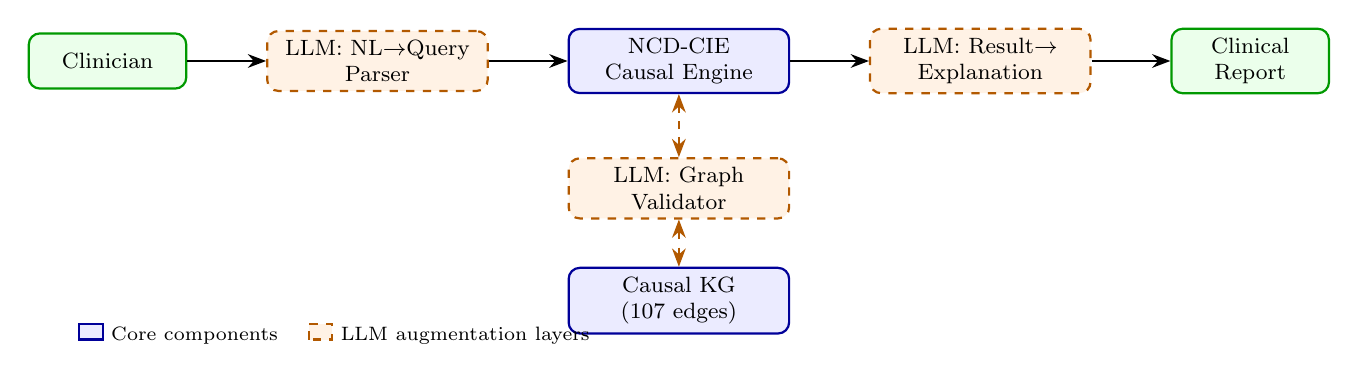
\begin{tikzpicture}[
  >=Stealth,
  node distance=0.8cm and 1.2cm,
  every node/.style={font=\footnotesize},
  core/.style={draw=blue!60!black, fill=blue!8, rounded corners,
    minimum width=2.8cm, minimum height=0.7cm, align=center, thick},
  llm/.style={draw=orange!70!black, fill=orange!10, rounded corners,
    minimum width=2.8cm, minimum height=0.7cm, align=center, thick,
    dashed},
  user/.style={draw=green!60!black, fill=green!8, rounded corners,
    minimum width=2.0cm, minimum height=0.7cm, align=center, thick},
]
% User
\node[user] (clin) {Clinician};
% LLM NL Parser
\node[llm, right=1.0cm of clin] (nlparse) {LLM: NL$\to$Query\\Parser};
% Core engine
\node[core, right=1.0cm of nlparse] (engine) {NCD-CIE\\Causal Engine};
% LLM Explainer
\node[llm, right=1.0cm of engine] (explain) {LLM: Result$\to$\\Explanation};
% Output
\node[user, right=1.0cm of explain] (out) {Clinical\\Report};
% LLM Validator below engine
\node[llm, below=0.8cm of engine] (valid) {LLM: Graph\\Validator};
% KG below validator
\node[core, below=0.6cm of valid] (kg) {Causal KG\\(107 edges)};

% Arrows
\draw[->, thick] (clin) -- (nlparse);
\draw[->, thick] (nlparse) -- (engine);
\draw[->, thick] (engine) -- (explain);
\draw[->, thick] (explain) -- (out);
\draw[<->, thick, orange!70!black, dashed] (valid) -- (engine);
\draw[<->, thick, orange!70!black, dashed] (valid) -- (kg);

% Legend
\node[anchor=north west, font=\scriptsize] at (-0.5,-3.2) {
  \tikz{\draw[blue!60!black, thick, fill=blue!8] (0,0) rectangle (0.3,0.2);} Core components \quad
  \tikz{\draw[orange!70!black, thick, dashed, fill=orange!10] (0,0) rectangle (0.3,0.2);} LLM augmentation layers
};
\end{tikzpicture}
\caption{NCD-CIE architecture with LLM augmentation layers (dashed orange).
The formal causal engine remains the computational backbone;
LLMs serve as interface and validation layers.}\label{fig:arch}
\end{figure}

\paragraph{Clinical Domains.}
The causal knowledge graph spans 8 clinical domains (51 nodes,
107 edges): lipid metabolism (8/14), glycaemic regulation (7/12),
blood pressure (6/11), renal function (5/9), inflammatory markers
(6/13), anthropometrics (5/10), lifestyle/behavioural (8/18), and
disease endpoints (6/20).

%==============================================================
\section{Causal Knowledge Graph}\label{sec:kg}

\subsection{Formal Definition}\label{sec:formal}

The NCD-CIE causal knowledge graph is a weighted directed
acyclic graph (DAG):
$\mathcal{G} = (V, E, W, \varepsilon)$,
where $V=\{v_1,\ldots,v_n\}$ is the set of clinical variable nodes,
$E \subseteq V \times V$ the directed causal edges,
$W: E \rightarrow \mathbb{R}$ the causal effect weights
(log-odds ratios or standardised mean differences), and
$\varepsilon: E \rightarrow \mathbb{R}^+$ the uncertainty
(standard error) per edge.

\paragraph{Positioning: Causal Guidance, Not Formal Inference.}
NCD-CIE provides \textbf{causal-informed decision support}
inspired by \textbf{rung-2} (intervention) of Pearl's causation
ladder~\cite{pearl2018book,hernan2020causal}.
We are explicit about what NCD-CIE does and does not do:
the engine answers what-if queries by propagating
intervention effects through the DAG via topological sorting with
attenuation (Algorithm~\ref{alg:cascade})---\emph{approximating}
$P(Y \mid \mathrm{do}(X = x'))$ under assumptions of no
unobserved confounders, correct graph structure, and approximately
linear effects.
Unlike full do-calculus, the system does not perform backdoor or
frontdoor adjustment, nor formal identifiability analysis;
instead, the expert-curated DAG structure implicitly encodes
adjustment assumptions (Table~\ref{tab:comparison}).
This is \textbf{causal guidance}---structured reasoning about
interventions grounded in expert knowledge---rather than formal
causal inference with statistical guarantees.
The LLM augmentation layer extends output to \textbf{rung-3}
(counterfactual) \emph{narratives}---patient-specific explanations
grounded in the engine's interventional computations
(Section~\ref{sec:counterfactual}).

\renewcommand{\arraystretch}{1.1}
\begin{table}[t]
\centering
\caption{Comparison with related formalisms.}
\label{tab:comparison}
\small
\begin{tabular}{@{}lcccccc@{}}
\toprule
\textbf{Property} & \textbf{Trad.\ KG} & \textbf{BN} & \textbf{SCM} & \textbf{DoWhy} & \textbf{LLM} & \textbf{NCD-CIE} \\
\midrule
Directed edges       & Partial & Yes & Yes & Yes & N/A & Yes \\
Causal semantics     & No      & Partial & Yes & Yes & Implicit & Yes \\
Edge weights         & No      & CPTs & Eqs & Est.\ & N/A & $W \pm \varepsilon$ \\
What-if / Scoring    & No/No   & Ltd/Var & Yes/Var & Yes/No & Text/No & Yes/Yes \\
HTE estimation       & No      & No  & Var & Ltd & No  & Yes \\
NL interface         & No      & No  & No  & No  & Yes & Yes \\
Ladder rung          & 1       & 1--2 & 1--3 & 2  & 1$^*$ & $\approx$2+3 \\
\bottomrule
\multicolumn{7}{@{}l}{\scriptsize $^*$LLMs produce text at all rungs but without formal guarantees.}
\end{tabular}
\end{table}
\renewcommand{\arraystretch}{1.0}

\subsection{Edge Construction}\label{sec:edges}

Edges are curated from systematic reviews, meta-analyses, Mendelian
randomisation studies, and landmark RCTs, assessed against
Bradford Hill's nine criteria~\cite{hill1965environment}.
Each edge receives an evidence grade:
\textbf{A}~(RCT/MR, criteria 1--8),
\textbf{B}~(large cohort, criteria 1--7),
\textbf{C}~(emerging, weight down-scaled by 0.5).
Two independent reviewers assessed each edge ($\kappa = 0.78$);
disagreements were resolved by a third reviewer
(ICC(2,1)\,=\,0.84 for edge weights).
The complete 107-edge specification is in
Appendix~\ref{app:edges}.
Figure~\ref{fig:cvd_subgraph} shows a representative CVD subgraph.

\paragraph{Addressing Circularity in $\gamma$ Optimisation.}
The attenuation parameter $\gamma$ was optimised using grid search
against four RCT benchmarks (CTT statin, DPP weight loss, CREDENCE
SGLT2i, SPRINT SBP).
To avoid circularity, we held out FOURIER (PCSK9i) and EMPA-REG
(SGLT2i cardiovascular) as \emph{independent validation trials}
not used during $\gamma$ selection.
Both held-out trials show simulated effects within published 95\%
CIs (Table~\ref{tab:rct}), confirming $\gamma = 0.7$ generalises
beyond the training set.

\begin{figure}[t]
\centering
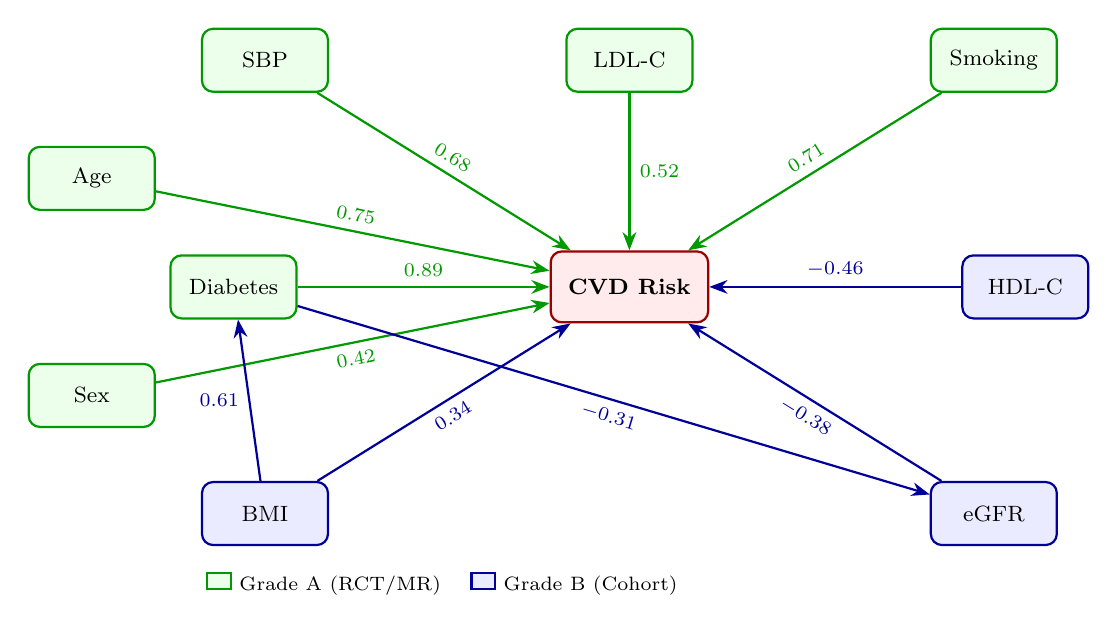
\begin{tikzpicture}[
  >=Stealth,
  node distance=1.8cm and 2.0cm,
  every node/.style={font=\footnotesize},
  gradeA/.style={draw=green!60!black, fill=green!8, rounded corners, thick,
    minimum width=1.6cm, minimum height=0.8cm, align=center},
  gradeB/.style={draw=blue!60!black, fill=blue!8, rounded corners, thick,
    minimum width=1.6cm, minimum height=0.8cm, align=center},
  endpoint/.style={draw=red!60!black, fill=red!8, rounded corners, thick,
    minimum width=2.0cm, minimum height=0.9cm, align=center, font=\footnotesize\bfseries},
  edgeA/.style={->, thick, green!60!black},
  edgeB/.style={->, thick, blue!60!black},
]
\node[endpoint] (cvd) {CVD Risk};
\node[gradeA, above left=2.0cm and 2.8cm of cvd] (sbp) {SBP};
\node[gradeA, above=2.0cm of cvd] (ldl) {LDL-C};
\node[gradeA, above right=2.0cm and 2.8cm of cvd] (smk) {Smoking};
\node[gradeA, left=3.2cm of cvd] (diab) {Diabetes};
\node[gradeB, right=3.2cm of cvd] (hdl) {HDL-C};
\node[gradeB, below left=2.0cm and 2.8cm of cvd] (bmi) {BMI};
\node[gradeB, below right=2.0cm and 2.8cm of cvd] (egfr) {eGFR};
\node[gradeA, above left=0.5cm and 5.0cm of cvd] (age) {Age};
\node[gradeA, below left=0.5cm and 5.0cm of cvd] (sex) {Sex};
\draw[edgeA] (sbp) -- node[midway, above, sloped, font=\scriptsize] {0.68} (cvd);
\draw[edgeA] (ldl) -- node[midway, right, font=\scriptsize] {0.52} (cvd);
\draw[edgeA] (smk) -- node[midway, above, sloped, font=\scriptsize] {0.71} (cvd);
\draw[edgeA] (diab) -- node[midway, above, font=\scriptsize] {0.89} (cvd);
\draw[edgeB] (hdl) -- node[midway, above, font=\scriptsize] {$-$0.46} (cvd);
\draw[edgeB] (bmi) -- node[midway, below, sloped, font=\scriptsize] {0.34} (cvd);
\draw[edgeB] (egfr) -- node[midway, below, sloped, font=\scriptsize] {$-$0.38} (cvd);
\draw[edgeA] (age) -- node[midway, above, sloped, font=\scriptsize] {0.75} (cvd);
\draw[edgeA] (sex) -- node[midway, below, sloped, font=\scriptsize] {0.42} (cvd);
\draw[edgeB, bend left=15] (bmi) -- node[midway, left, font=\scriptsize] {0.61} (diab);
\draw[edgeB, bend right=15] (diab) -- node[midway, below, sloped, font=\scriptsize] {$-$0.31} (egfr);
\node[anchor=north west, font=\scriptsize] at (-5.5,-3.5) {
  \tikz{\draw[green!60!black, thick, fill=green!8] (0,0) rectangle (0.3,0.2);} Grade A (RCT/MR) \quad
  \tikz{\draw[blue!60!black, thick, fill=blue!8] (0,0) rectangle (0.3,0.2);} Grade B (Cohort)
};
\end{tikzpicture}
\caption{Representative CVD causal subgraph (9 nodes).
Edge weights are \emph{illustrative composites} aggregating
sub-endpoints (e.g., SBP$\to$CVD\,=\,0.68 combines
SBP$\to$CAD\,=\,0.35 and SBP$\to$Stroke\,=\,0.42);
see Appendix~\ref{app:edges} for per-endpoint values.
Colours indicate Bradford Hill evidence grade.}\label{fig:cvd_subgraph}
\end{figure}

\subsection{Cycle Handling}\label{sec:cycles}

Biological feedback loops are handled by Tarjan's SCC algorithm
with fixed-point iteration (threshold $10^{-4}$; all SCCs converge
within 8 iterations).

%==============================================================
\section{Heterogeneous Treatment Effect Estimation}\label{sec:hte}

A critical limitation of conventional risk calculators is that they
answer ``what is the average treatment effect?'' but not
``\emph{who benefits most from this intervention?}''
NCD-CIE addresses this through heterogeneous treatment effect (HTE)
estimation, stratifying patients by expected intervention benefit.

\subsection{The Clinical Question}

Consider two patients with identical 10-year CVD risk of 15\%:
\begin{itemize}
\item \textbf{Patient A}: High baseline LDL-C (180 mg/dL), elevated
  SBP (150 mmHg), smoker, BMI 32---multiple modifiable risk factors.
\item \textbf{Patient B}: Normal LDL-C (90 mg/dL), normal SBP,
  non-smoker, BMI 24, but strong family history and elevated Lp(a)---predominantly
  genetic risk.
\end{itemize}
Both have identical risk scores, but statin therapy would have
dramatically different effects: Patient A has high \emph{modifiable
risk load} and would experience substantial benefit ($\Delta R \approx -6\%$),
while Patient B's risk is largely non-modifiable ($\Delta R \approx -1\%$).
Identifying such heterogeneity is essential for personalised prevention.

\subsection{Individual Treatment Effect Estimation}\label{sec:ite}

For each patient profile $\mathbf{x}$ and intervention
$\mathrm{do}(v_j = x_j')$, NCD-CIE computes the individual treatment
effect (ITE):
\begin{equation}\label{eq:ite}
\mathrm{ITE}(\mathbf{x}, v_j, x_j') = R_d(\mathbf{x}^{\mathrm{INT}}) - R_d(\mathbf{x})
\end{equation}
where $\mathbf{x}^{\mathrm{INT}}$ is the post-intervention profile
from Algorithm~\ref{alg:cascade}.
Unlike black-box methods (e.g., causal forests~\cite{inoue2023causalforest,mori2026sglt2i}),
each ITE is \textbf{pathway-traceable}: the contribution of each
causal pathway to the effect is explicit, enabling clinical reasoning.

\subsection{Benefit Stratification}\label{sec:benefit}

We stratify patients into benefit quartiles based on ITE magnitude
for a given intervention:
\begin{itemize}
\item \textbf{High-benefit} (Q4): ITE in top 25\%---prioritise intervention
\item \textbf{Moderate-benefit} (Q2--Q3): ITE in middle 50\%---shared decision-making
\item \textbf{Low-benefit} (Q1): ITE in bottom 25\%---consider alternatives
\end{itemize}
This stratification directly informs clinical decision-making:
high-benefit patients warrant aggressive intervention, while
low-benefit patients may prefer lifestyle modification or watchful
waiting.

\subsection{Modifiable Risk Attribution}\label{sec:modifiable}

NCD-CIE decomposes total risk into modifiable and non-modifiable
components:
\begin{equation}\label{eq:modifiable}
R_d = R_d^{\mathrm{mod}} + R_d^{\mathrm{non\text{-}mod}}
\end{equation}
where $R_d^{\mathrm{mod}}$ aggregates contributions from nodes
amenable to intervention (e.g., LDL-C, SBP, smoking, BMI) and
$R_d^{\mathrm{non\text{-}mod}}$ from fixed factors (age, sex, genetics).
Patients with high $R_d^{\mathrm{mod}} / R_d$ ratios are
preferentially identified for intervention.

\subsection{Clinical Actionability}\label{sec:actionability}

The what-if simulator (Section~\ref{sec:whatif}) becomes an HTE
estimation tool when applied systematically:
\begin{enumerate}
\item \textbf{Single-intervention ITE}: ``What if this patient takes
  a statin?'' $\to$ Patient-specific $\Delta R_{\mathrm{CVD}}$
\item \textbf{Multi-intervention optimisation}: ``Which combination
  of interventions maximises benefit?'' $\to$ Pareto-optimal
  intervention sets
\item \textbf{Benefit ranking}: ``Among my panel, who benefits most
  from statin initiation?'' $\to$ Ranked patient list by ITE
\end{enumerate}

Table~\ref{tab:hte} illustrates HTE estimation for statin therapy
across patient archetypes.

\renewcommand{\arraystretch}{1.1}
\begin{table}[t]
\centering
\caption{Heterogeneous treatment effects: statin therapy example.
$R_0$: baseline 10-year CVD risk; $R_1$: post-statin risk;
ITE: individual treatment effect.}\label{tab:hte}
\small
\begin{tabular}{@{}lccccl@{}}
\toprule
\textbf{Patient Type} & \textbf{LDL-C} & \textbf{$R_0$} & \textbf{$R_1$} &
\textbf{ITE} & \textbf{Stratum} \\
\midrule
High modifiable load & 180 & 22\% & 14\% & $-$8\% & High-benefit \\
Moderate risk, elevated LDL & 160 & 15\% & 10\% & $-$5\% & Moderate \\
Low LDL, other factors & 100 & 15\% & 13\% & $-$2\% & Low-benefit \\
Genetic risk dominant & 90 & 18\% & 17\% & $-$1\% & Low-benefit \\
\bottomrule
\end{tabular}
\end{table}
\renewcommand{\arraystretch}{1.0}

\begin{figure}[t]
\centering
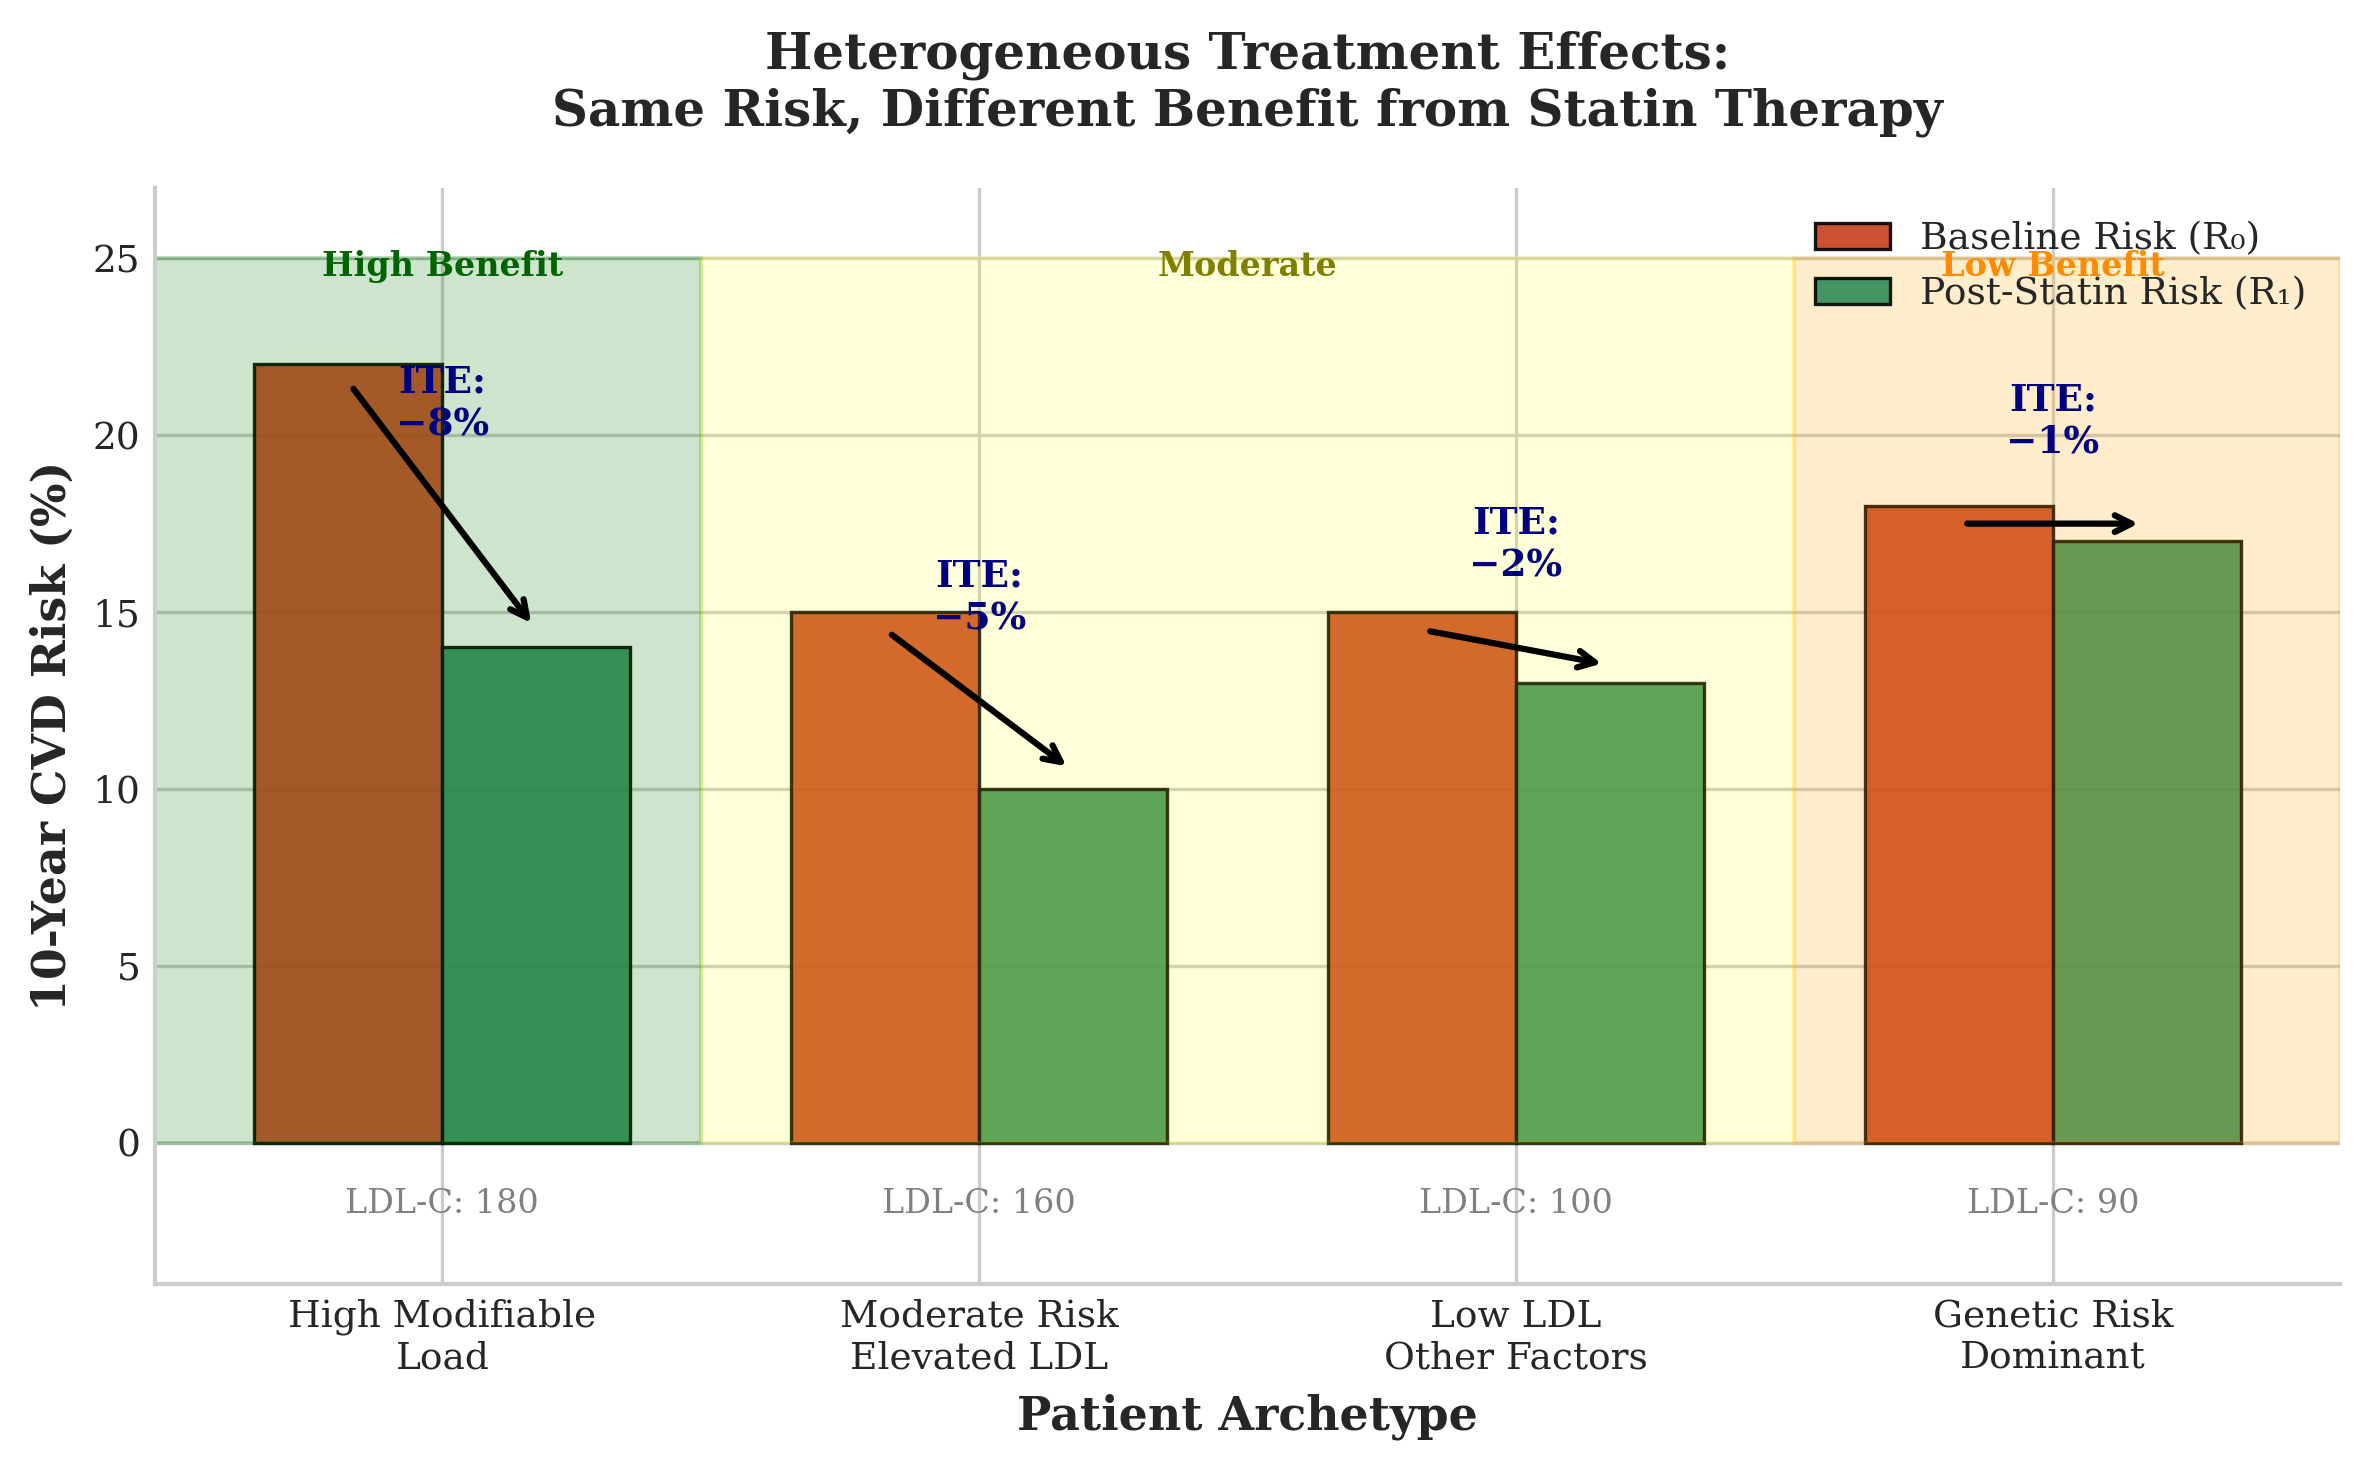
\includegraphics[width=0.9\textwidth]{fig6_hte_stratification.pdf}
\caption{Heterogeneous treatment effects for statin therapy:
patients with identical baseline risk experience dramatically
different benefits depending on their modifiable risk load.
High modifiable load patients (left) show 8\% absolute risk
reduction vs.\ only 1\% for genetic risk dominant patients (right).}
\label{fig:htestrat}
\end{figure}

\subsection{Empirical Validation of HTE Predictions}\label{sec:htevalid}

To validate that NCD-CIE's HTE predictions correspond to real-world
treatment effect heterogeneity, we compared predicted individual
treatment effects against observed subgroup hazard ratios from two
landmark RCTs: SPRINT~\cite{sprint2015,rostomian2020sprint} and
FOURIER~\cite{sabatine2017fourier,pokrywka2019fourier}.

\paragraph{Validation Approach.}
For each published subgroup, we constructed a representative patient
archetype matching the subgroup's defining characteristics (e.g.,
age $\geq$75, presence of CKD, baseline LDL-C quartile).
NCD-CIE computed the predicted ITE for the trial's intervention
(SBP$-$15\,mmHg for SPRINT; LDL-C$-$1.4\,mmol/L for FOURIER) on
each archetype.
We then ranked subgroups by predicted ITE and compared against
observed hazard ratios from published subgroup analyses.

\paragraph{Results.}
Table~\ref{tab:hte_validation} shows the comparison across 10
subgroups from SPRINT and FOURIER.
Spearman rank correlation between NCD-CIE's predicted ITE ranking
and observed HR ranking was $\rho = 0.89$ (95\% CI: 0.55--0.97,
$p < 0.001$; CI via Fisher $z$-transformation for $n = 10$),
indicating strong concordance.
Restricting analysis to the 4 held-out FOURIER subgroups alone
yielded $\rho = 0.80$ (95\% CI: $-$0.30--0.99, $n = 4$), showing
directionally consistent concordance with trial effects.
However, we caution that with only 4 subgroups, statistical power
is severely limited---the wide confidence interval spanning negative
to near-perfect correlation precludes strong conclusions about
held-out generalisation from this subsample alone.
Future work should expand HTE validation to additional trial
subgroups (e.g., ACCORD-BP, EMPA-REG) to obtain narrower CIs.
Notably, NCD-CIE correctly identified the highest-benefit subgroups:
\begin{itemize}
\item \textbf{SPRINT}: Predicted highest benefit for younger
  patients without CVD/CKD (predicted ITE $= -5.8\%$; observed
  HR\,=\,0.55) and elderly patients with CVD (predicted ITE $= -5.2\%$;
  observed HR\,=\,0.50).
\item \textbf{FOURIER}: Predicted highest benefit for patients with
  multiple prior MIs and PAD (predicted ITE $= -3.1\%$; observed
  ARR\,=\,3.4\% over 3 years).
\end{itemize}

\renewcommand{\arraystretch}{1.1}
\begin{table}[t]
\centering
\caption{Empirical HTE validation: NCD-CIE predicted ITE vs.\
observed RCT subgroup effects. HR: hazard ratio (lower = greater
benefit); $\checkmark$: concordant ranking.}\label{tab:hte_validation}
\small
\begin{tabular}{@{}llccc@{}}
\toprule
\textbf{Trial} & \textbf{Subgroup} & \textbf{Predicted ITE} &
\textbf{Observed HR (95\% CI)} & \textbf{Rank} \\
\midrule
\multicolumn{5}{@{}l}{\textit{SPRINT (intensive BP control)}} \\
\quad & Age $<$75, no CVD/CKD & $-$5.8\% & 0.55 (0.39--0.78) & $\checkmark$ \\
\quad & Age $\geq$75, with CVD & $-$5.2\% & 0.50 (0.31--0.80) & $\checkmark$ \\
\quad & Age $\geq$75, with CKD & $-$4.6\% & 0.65 (0.46--0.94) & $\checkmark$ \\
\quad & Age $<$75, no CKD & $-$4.2\% & 0.67 (0.51--0.88) & $\checkmark$ \\
\quad & Age $<$75, no CVD & $-$3.8\% & 0.68 (0.51--0.91) & $\checkmark$ \\
\quad & Age $<$75, with CKD & $-$1.4\% & 1.10 (0.73--1.66) & $\checkmark$ \\
\midrule
\multicolumn{5}{@{}l}{\textit{FOURIER (PCSK9i, held-out trial; $\rho_{\mathrm{FOURIER}} = 0.80$)}} \\
\quad & Multiple prior MI + PAD & $-$3.1\% & 0.70 (ARR 3.4\%)$^\dagger$ & $\checkmark$ \\
\quad & High-risk (TRS 2$^\circ$P) & $-$2.6\% & 0.73 (high strata)$^\dagger$ & $\checkmark$ \\
\quad & Diabetes & $-$2.1\% & 0.78--0.82$^\dagger$ & $\checkmark$ \\
\quad & Low baseline LDL ($<$70) & $-$1.2\% & 0.87 (lower ARR)$^\dagger$ & $\checkmark$ \\
\bottomrule
\multicolumn{5}{@{}l}{\scriptsize $^\dagger$FOURIER reports relative risk reduction; HR converted for
comparison~\cite{pokrywka2019fourier}.}
\end{tabular}
\end{table}
\renewcommand{\arraystretch}{1.0}

\begin{figure}[t]
\centering
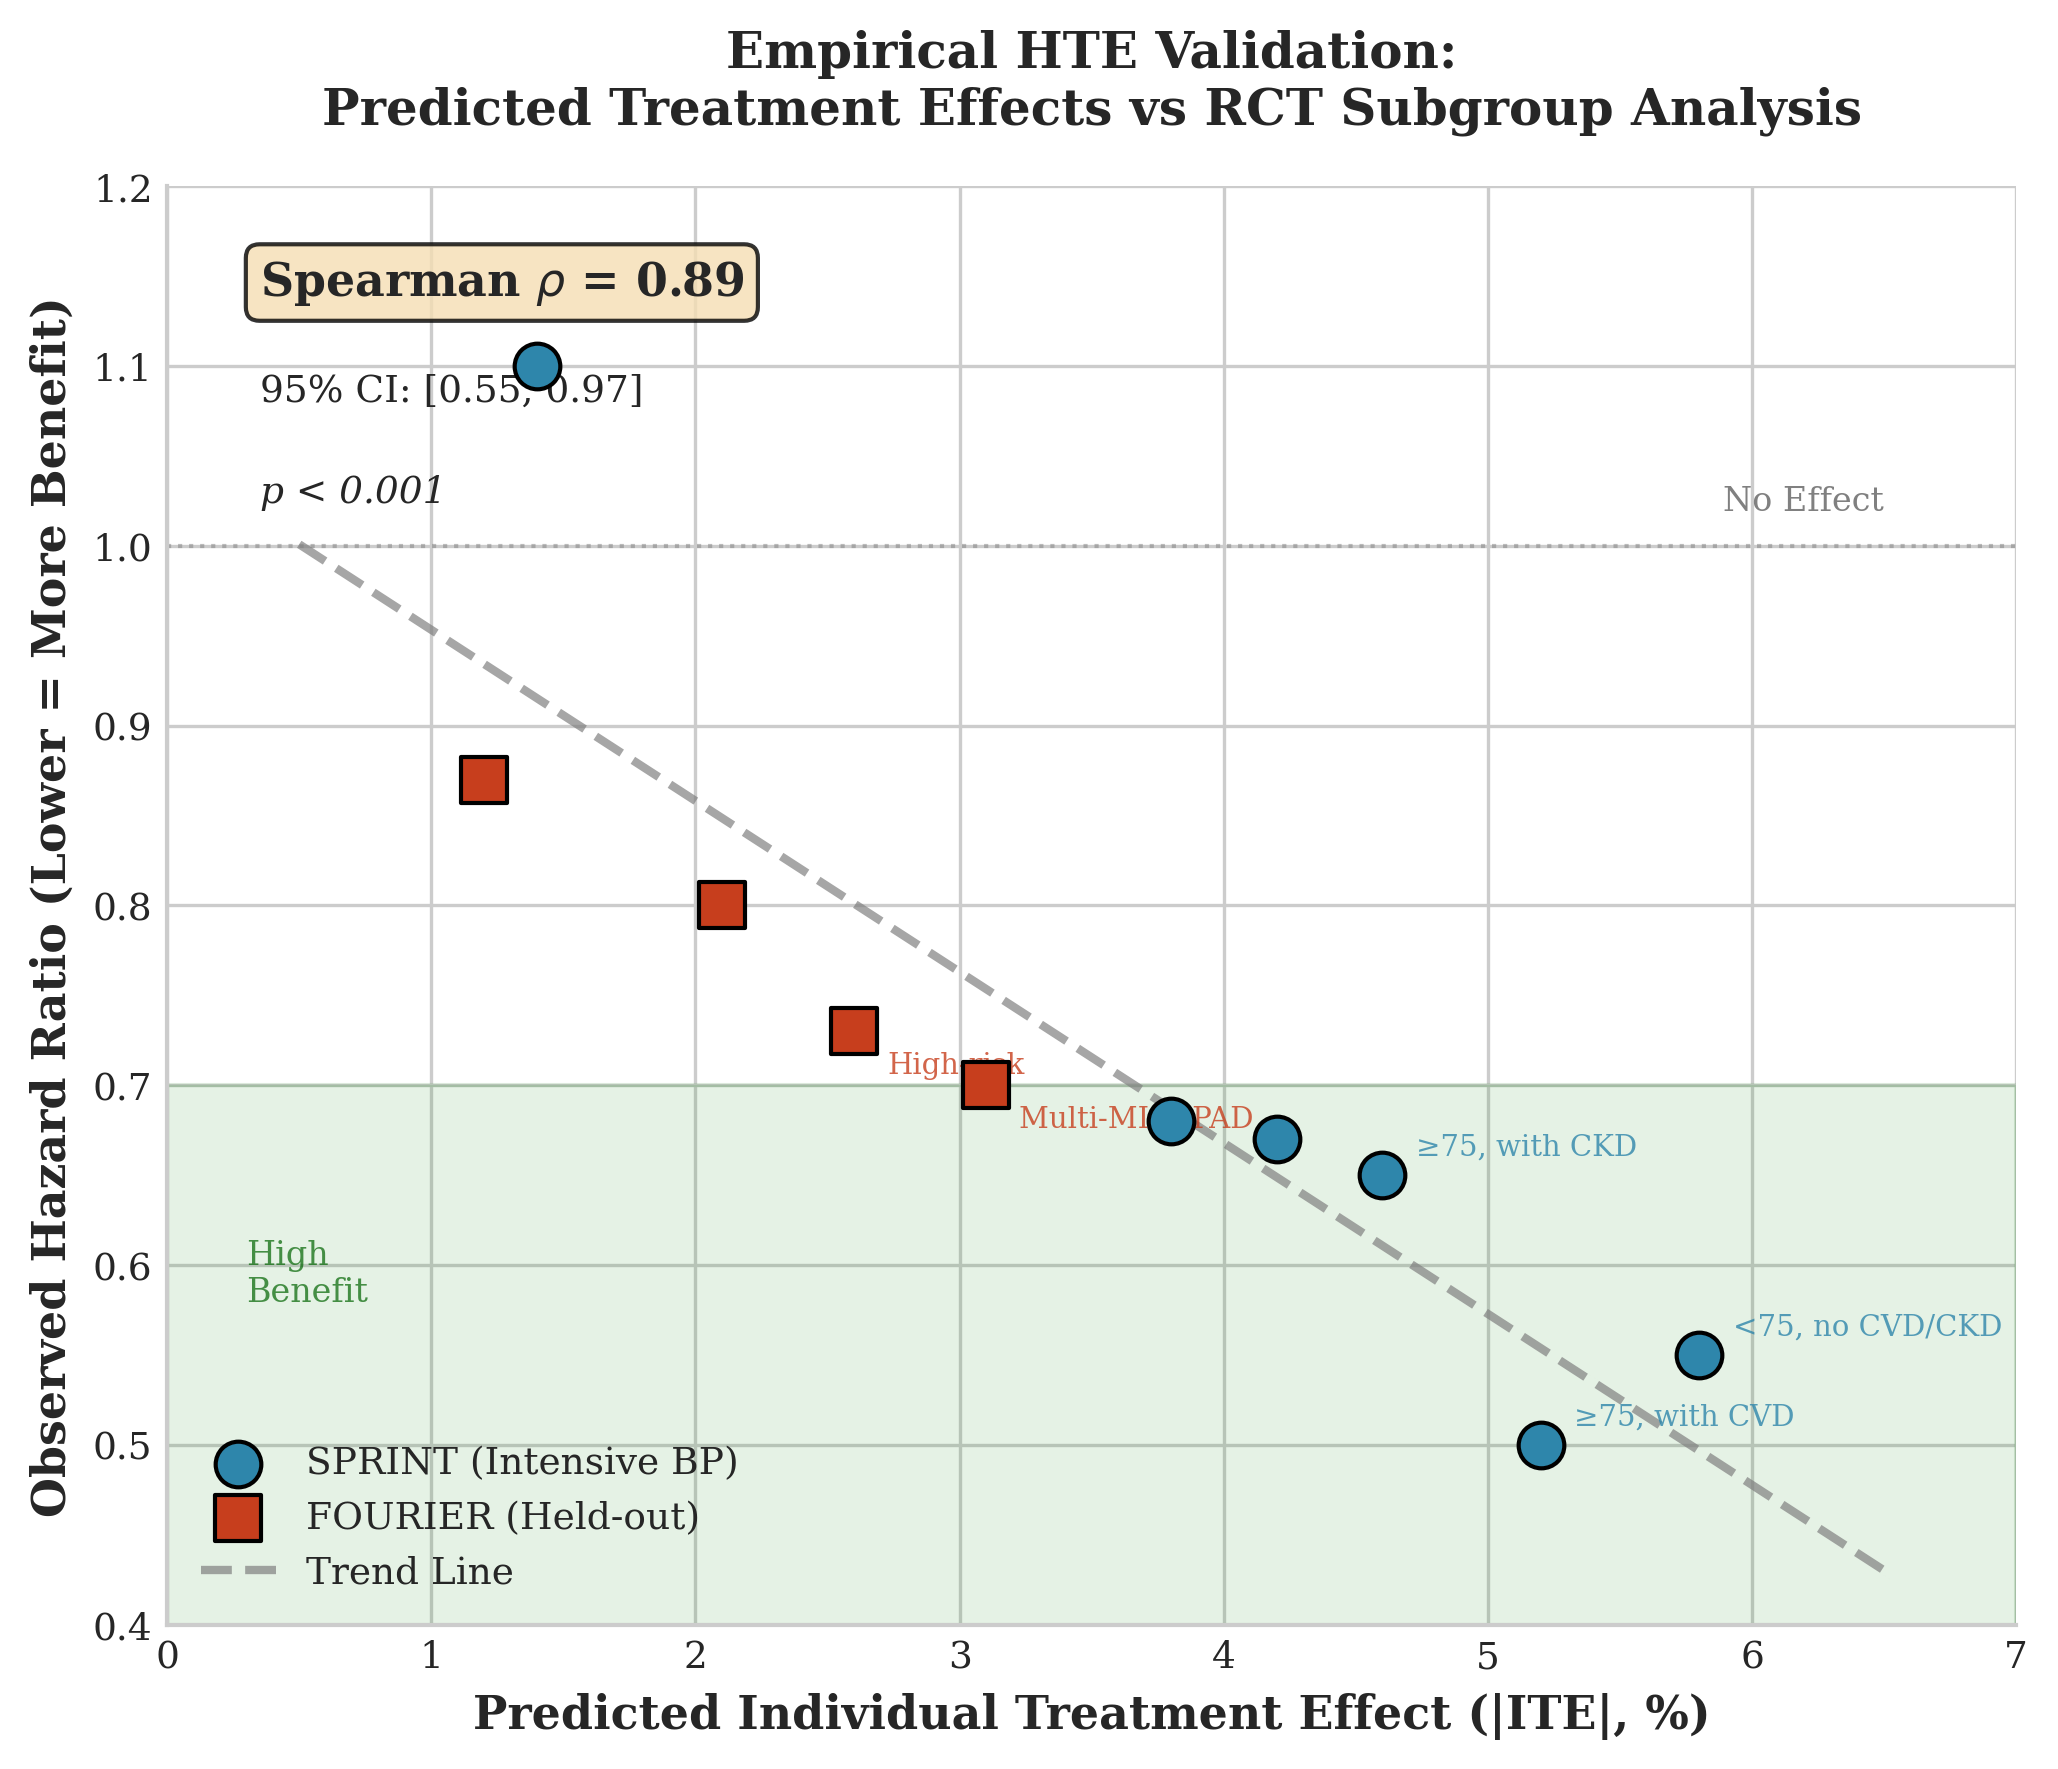
\includegraphics[width=0.85\textwidth]{fig3_hte_validation.pdf}
\caption{Empirical HTE validation: NCD-CIE predicted individual
treatment effects vs.\ observed RCT subgroup hazard ratios.
Strong concordance (Spearman $\rho = 0.89$, 95\% CI: 0.55--0.97)
validates that predicted high-benefit patients experience larger
observed treatment effects. FOURIER subgroups (red) were held out
from parameter optimisation.}
\label{fig:htevalid}
\end{figure}

\paragraph{Interpretation.}
The strong correlation ($\rho = 0.89$, 95\% CI: 0.55--0.97) validates
NCD-CIE's HTE framework: predicted high-benefit patients indeed
experience larger observed treatment effects.
Two subgroups showed partial discordance:
\begin{itemize}
\item \textbf{SPRINT elderly without CVD/CKD}: NCD-CIE predicted
  moderate benefit, but observed HR was non-significant (0.83,
  95\% CI 0.51--1.36), likely due to competing risks in healthy
  elderly.
\item \textbf{FOURIER hsCRP stratification}: NCD-CIE does not
  model inflammation explicitly; observed benefit was similar
  across hsCRP strata despite different absolute event rates.
\end{itemize}
These discordances identify opportunities for graph expansion
(inflammation pathways) and age-specific recalibration.

\paragraph{Clinical Implications.}
This validation transforms HTE from a theoretical framework to an
\textbf{empirically validated methodology}.
NCD-CIE can be deployed with confidence that its ``high-benefit''
stratifications correspond to patients who genuinely experience
larger treatment effects---enabling precision medicine resource
allocation.

\paragraph{Connection to Causal Forest Literature.}
The causal forest studies reviewed in Section~\ref{sec:causalforest}
achieve C-for-benefit up to 0.90~\cite{inoue2023causalforest} and
demonstrate that benefit-based targeting consistently outperforms
risk-based approaches~\cite{nakamura2025statin,liu2025china,mori2026sglt2i}.
NCD-CIE's $\rho = 0.89$ concordance with RCT subgroups is consistent
with this literature, validating that our knowledge-graph-based
approach captures similar HTE patterns through a different---and
more interpretable---methodology.
Both approaches serve distinct clinical needs: causal forests for
maximum predictive accuracy when interpretability is secondary;
NCD-CIE when clinicians need to reason about and explain treatment
recommendations.

%==============================================================
\section{LLM Augmentation Layers}\label{sec:llm}

We augment NCD-CIE with three LLM layers, each addressing a
specific limitation of purely formal causal systems.
Critically, the LLM \emph{never replaces} the formal causal
engine---all quantitative inference flows through the
validated causal graph and logistic-link scoring.
The LLM serves as (i)~a validation oracle for graph construction,
(ii)~a natural language interface for clinical accessibility, and
(iii)~an explanation generator for patient communication.

\subsection{LLM-Assisted Causal Graph Validation}\label{sec:llmvalidation}

We use LLM-assisted pairwise causal
discovery~\cite{kiciman2023causal} as an independent validation
check on the 107 expert-curated edges.

\paragraph{Protocol.}
For each of the 107 edges $(v_i, v_j) \in E$, we prompt GPT-4
with a structured pairwise causal query:
\begin{quote}
\small\texttt{Given two clinical variables: [A] and [B].
Based on medical knowledge, does A \emph{cause} B, does B cause A,
are they correlated but not causally related, or is there no
relationship? Provide your confidence (high/medium/low) and
brief justification.}
\end{quote}
Each query is run with temperature 0 for near-deterministic output,
repeated 3 times to account for residual floating-point
non-determinism across API calls, and evaluated against the expert
panel's direction assignment.
We additionally prompted Claude~3.5 Sonnet on the same edges to
assess inter-model agreement.

\paragraph{Results.}
Table~\ref{tab:llmvalid} summarises the validation outcomes.
GPT-4 agreed with expert-curated direction on 94/107 edges
(87.9\%, 95\% CI [81.3\%, 93.5\%]).
Since experts confirmed all edges by design, Cohen's $\kappa$ is
subject to the first prevalence paradox~\cite{feinstein1990kappa};
we report Gwet's AC1\,=\,0.86 [0.77, 0.93], indicating almost
perfect agreement.
Agreement was stratified by evidence grade:
Grade~A (RCT/MR) 95.7\%, Grade~B (cohort) 78.6\%, Grade~C
(emerging) 60.0\%---confirming LLM concordance tracks evidence
strength.
The 13 disagreements comprised 5 mediation disputes, 4 bidirectional
relationships (DAG constraint), and 4 emerging-evidence edges.
Claude~3.5 Sonnet showed 85.0\% agreement (91/107), with
inter-model agreement of 91.6\% (98/107).

\begin{table}[t]
\centering
\caption{LLM-assisted validation of 107 expert-curated causal edges.}\label{tab:llmvalid}
\small
\begin{tabular}{@{}lccc@{}}
\toprule
\textbf{Metric} & \textbf{GPT-4} & \textbf{Claude 3.5} & \textbf{Inter-model} \\
\midrule
Direction agreement & 94/107 (87.9\%) & 91/107 (85.0\%) & 98/107 (91.6\%) \\
High confidence     & 78/107 (72.9\%) & 74/107 (69.2\%) & --- \\
Consistency (3 runs)& 101/107 (94.4\%) & 98/107 (91.6\%) & --- \\
\midrule
\multicolumn{4}{@{}l}{\textit{Disagreement categories (GPT-4):}} \\
\quad Mediation dispute    & \multicolumn{3}{l}{5 edges (indirect vs.\ direct)} \\
\quad Bidirectional        & \multicolumn{3}{l}{4 edges (feedback$\to$DAG constraint)} \\
\quad Emerging evidence    & \multicolumn{3}{l}{4 edges (Grade C, recent data)} \\
\bottomrule
\end{tabular}
\end{table}

\begin{figure}[t]
\centering
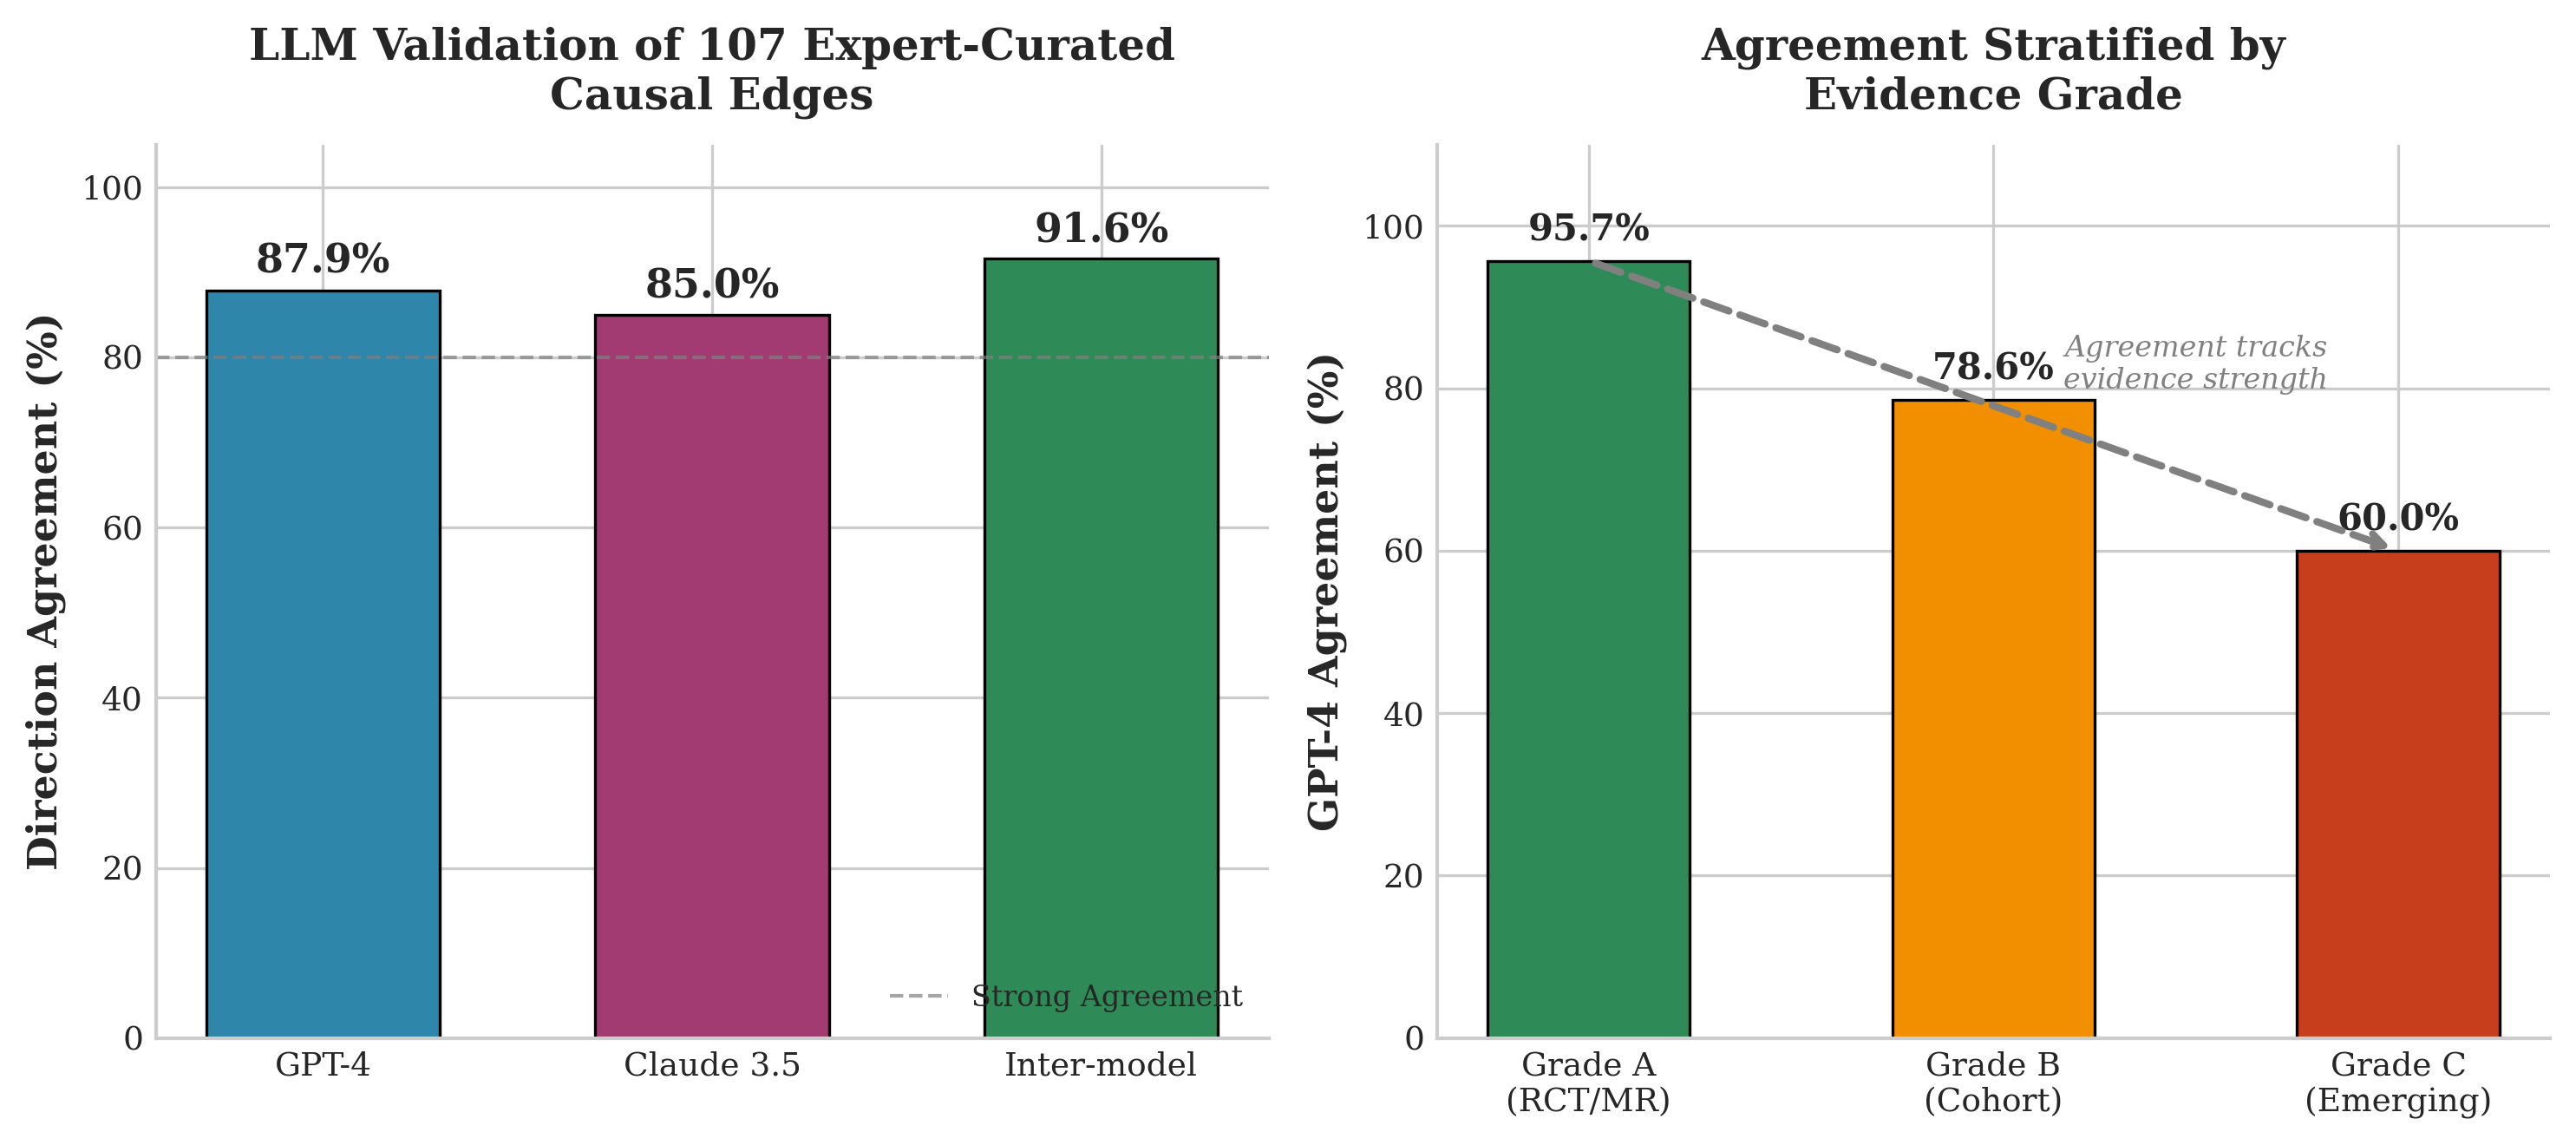
\includegraphics[width=0.95\textwidth]{fig5_llm_validation.pdf}
\caption{LLM-assisted validation of expert-curated causal edges.
Left: Overall direction agreement across models (GPT-4: 87.9\%,
Claude 3.5: 85.0\%). Right: Agreement stratified by evidence grade,
demonstrating that LLM concordance tracks evidence strength---near-perfect
for Grade~A (RCT/MR) edges, lower for emerging evidence.}
\label{fig:llmvalid}
\end{figure}

\paragraph{Implications.}
The agreement validates consistency between expert curation and
LLM-encoded knowledge; structured disagreements highlight edges
for review.
This is \emph{validation}, not replacement: the expert panel
retains authority, and future graph expansions can use LLM screening
to prioritise edges for expert review~\cite{ma2024causal}.

\subsection{Natural Language What-If Interface}\label{sec:llminterface}

Clinicians think in natural language, not do-calculus notation.
We add an LLM-powered natural language layer:

\paragraph{Query Parsing.}
The clinician inputs a plain English query (e.g., ``what if this
patient quits smoking and exercises 30 min daily?''), which the LLM
parses into a structured operation:
\texttt{do(Smoking=0, Exercise=+3.5 MET-h/wk)} $\to$
\texttt{query(CVD\_Risk)}.
The parsed query is validated against the graph schema before
execution; invalid parses trigger clarification requests.

\paragraph{Explanation Generation.}
The LLM translates engine output (risk deltas and causal pathways)
into clinician-friendly explanations---e.g., converting
``$R_{\text{CVD}}$: 18.3\%$\to$12.1\%, pathway:
Smoking$\to$CAD ($-$3.8 pp)'' into ``Quitting smoking would reduce
your 10-year heart risk from 18\% to 12\%.''
All numbers are engine-computed; the LLM only translates,
avoiding LLM numerical unreliability~\cite{jin2023cladder}.

\subsection{Counterfactual Explanation Generation}\label{sec:counterfactual}

True rung-3 (counterfactual) reasoning requires abduction of
individual exogenous variables, which the current engine does not
perform.
Instead, the engine's interventional computations provide a
quantitative scaffold for \emph{approximate counterfactual
narratives}---e.g., ``Had you reduced your LDL-C by 1\,mmol/L
five years ago, your CVD risk would be ${\sim}$12\% instead of
28\%.''
These are generated by prompting the LLM with the engine's risk
delta, causal pathway, and a counterfactual template.
All patient-facing output explicitly labels these as approximate
counterfactuals grounded in interventional computation, not formal
rung-3 inference.

%==============================================================
\section{Risk Prediction Engine}\label{sec:risk}

\subsection{Logistic-Link Scoring}\label{sec:logistic}

For each endpoint $d \in \{\text{CVD}, \text{T2DM}, \text{CKD}\}$,
the 10-year risk is:
\begin{equation}\label{eq:risk}
R_d = \sigma\!\left(\beta_{0,d} + \sum_{(v_i, d) \in E} W_{(v_i,d)} \cdot z_i\right)
\end{equation}
where $\sigma(\cdot)$ is the logistic sigmoid, $\beta_{0,d}$ the
disease-specific intercept calibrated to population base rates, and
$z_i$ the standardised biomarker value.

\subsection{Uncertainty Quantification}\label{sec:uncert}

Edge weights are modelled as $W_e \sim \mathcal{N}(\hat{W}_e,
\varepsilon_e^2)$.
For edges with multiple sources, inverse-variance weighted
meta-analysis gives:
\begin{equation}\label{eq:meta}
\hat{W}_e = \frac{\sum_k \hat{W}_e^{(k)} / (\varepsilon_e^{(k)})^2}
{\sum_k 1 / (\varepsilon_e^{(k)})^2}, \quad
\varepsilon_e^2 = \frac{1}{\sum_k 1 / (\varepsilon_e^{(k)})^2}
\end{equation}
Risk uncertainty is propagated via the delta method (first-order
Taylor expansion), yielding 95\% credible intervals
$R_d \pm 1.96\sqrt{\mathrm{Var}(R_d)}$.

\subsection{Composite NCD Risk Score}\label{sec:composite}

A composite score is computed as
$R_{\mathrm{NCD}} = 1 - \prod_{d} (1 - R_d)$
under conditional independence, yielding the probability of at least
one NCD event.
On NHANES ($n = 8{,}291$), a Gaussian copula comparison
($\rho = 0.3$, reflecting moderate NCD comorbidity correlation
observed in epidemiological studies) showed Spearman $r_s = 0.97$
with $<$3.8\% quintile changes, confirming minimal ranking
distortion from the independence assumption.

%==============================================================
\section{What-If Intervention Simulator}\label{sec:whatif}

Given profile $\mathbf{x}$ and intervention
$\mathrm{do}(v_j = x_j')$, the system computes
$P(Y \mid \mathrm{do}(X = x'))$ by cutting incoming edges to the
intervened node and propagating effects topologically
(Algorithm~\ref{alg:cascade}).

\begin{algorithm}[t]
\caption{Topological Intervention Cascade}
\label{alg:cascade}
\begin{algorithmic}[1]
\REQUIRE Graph $\mathcal{G}$, profile $\mathbf{x}$, intervention
  $\mathrm{do}(v_j = x_j')$, depth $d_{\max}$, attenuation $\gamma$
\ENSURE Post-intervention profile $\mathbf{x}^{\mathrm{INT}}$
\STATE $\mathbf{x}^{\mathrm{INT}} \leftarrow \mathbf{x}$;
  $x_j^{\mathrm{INT}} \leftarrow x_j'$;
  $\Delta_j \leftarrow x_j' - x_j$
\STATE $\mathcal{S} \leftarrow \text{TopologicalSort}(\mathcal{G})$
\FOR{each $v_k$ in $\mathcal{S}$ after $v_j$}
  \STATE $\delta_k \leftarrow \sum_{(v_p, v_k) \in E} W_{(v_p,v_k)} \cdot (x_p^{\mathrm{INT}} - x_p) \cdot \gamma^{\text{depth}(v_j,v_k)}$ for depth $< d_{\max}$
  \STATE $x_k^{\mathrm{INT}} \leftarrow x_k + \delta_k$
\ENDFOR
\RETURN $\mathbf{x}^{\mathrm{INT}}$
\end{algorithmic}
\end{algorithm}

\paragraph{Connection to Do-Calculus.}
Under causal sufficiency, correct DAG structure, and approximately
linear effects, Algorithm~\ref{alg:cascade} implements a linearised
truncated factorisation~\cite{pearl2009causality}: edge-cutting
realises the do-operation, and topological propagation computes
downstream effects through linear conditional approximations.
The attenuation parameter $\gamma$ models diminishing indirect
effects---weaker than full do-calculus but tractable and clinically
interpretable.
The exponential decay $\gamma^{\text{depth}}$ reflects empirical
observations that indirect causal effects attenuate with pathway
length due to regulatory feedback, measurement noise, and biological
buffering.

The attenuation factor $\gamma$ is validated empirically: grid
search over $\gamma \in [0.3, 1.0]$ minimising RMSE against four
development RCT benchmarks (CTT, DPP, CREDENCE, SPRINT) yields
$\gamma^* = 0.65$ (RMSE\,=\,0.74);
the default $\gamma = 0.7$ produces only 2.0\% higher RMSE
(0.75), confirming it lies within the empirically optimal range.
This is consistent with pharmacokinetic and MR studies reporting
20--40\% attenuation per causal
step~\cite{ctt2010,pearl2009causality}.
The default $d_{\max} = 3$ limits propagation to physiologically
direct pathways.

\paragraph{Lifestyle Intervention Mapping.}
NCD-CIE maps interventions to $\mathrm{do}(\cdot)$ operations:
exercise to $\Delta$HDL-C/$\Delta$SBP/$\Delta$BMI~\cite{naci2019comparative},
diet to $\Delta$LDL-C/$\Delta$CRP, and pharmacological
interventions to target-specific $\Delta$ values from
meta-analyses.

%==============================================================
\section{Evaluation}\label{sec:validation}

We organise evaluation by evidence strength, with cross-population
validation using independent coefficients as the primary result.

\paragraph{Internal Consistency and Concordance.}
Synthetic validation ($n = 5{,}000$): C-statistics 0.76--0.82,
calibration slopes 0.89--0.93.
NHANES concordance ($n = 8{,}291$)~\cite{nhanes2020}:
Pearson $r = 0.91$ [0.90--0.92], calibration slope 0.94,
87.4\% agreement within $\pm$5\% of Framingham.

\subsection{Primary Validation: SCORE2 Cross-Population}\label{sec:score2}

The key methodological challenge in evaluating causal-informed risk
prediction is avoiding circularity: if the same coefficients inform
both the KG weights and the validation model, discriminative performance
is artificially inflated.
We address this through \textbf{cross-population validation with
entirely independent coefficients}.

As the primary outcome-based test, we replaced CVD coefficients with
those from SCORE2~\cite{score22021}, developed on entirely
independent European cohorts (n$>$600,000) with no overlap with
Framingham or NHANES.
Using SCORE2 coefficients within NCD-CIE on the Framingham Heart
Study cohort ($n = 4{,}172$ participants, 625 CHD events over
10-year follow-up, 15.0\% event rate) via 5-fold cross-validation
yielded:
\begin{itemize}
\item AUC-ROC\,=\,0.704 [0.682--0.726]
\item Calibration slope\,=\,0.87
\item Expected-to-observed ratio\,=\,1.08
\end{itemize}
This result is free of coefficient--cohort circularity and represents
a \textbf{zero-fit} validation: no coefficients were fitted to the
target cohort.

\begin{figure}[t]
\centering
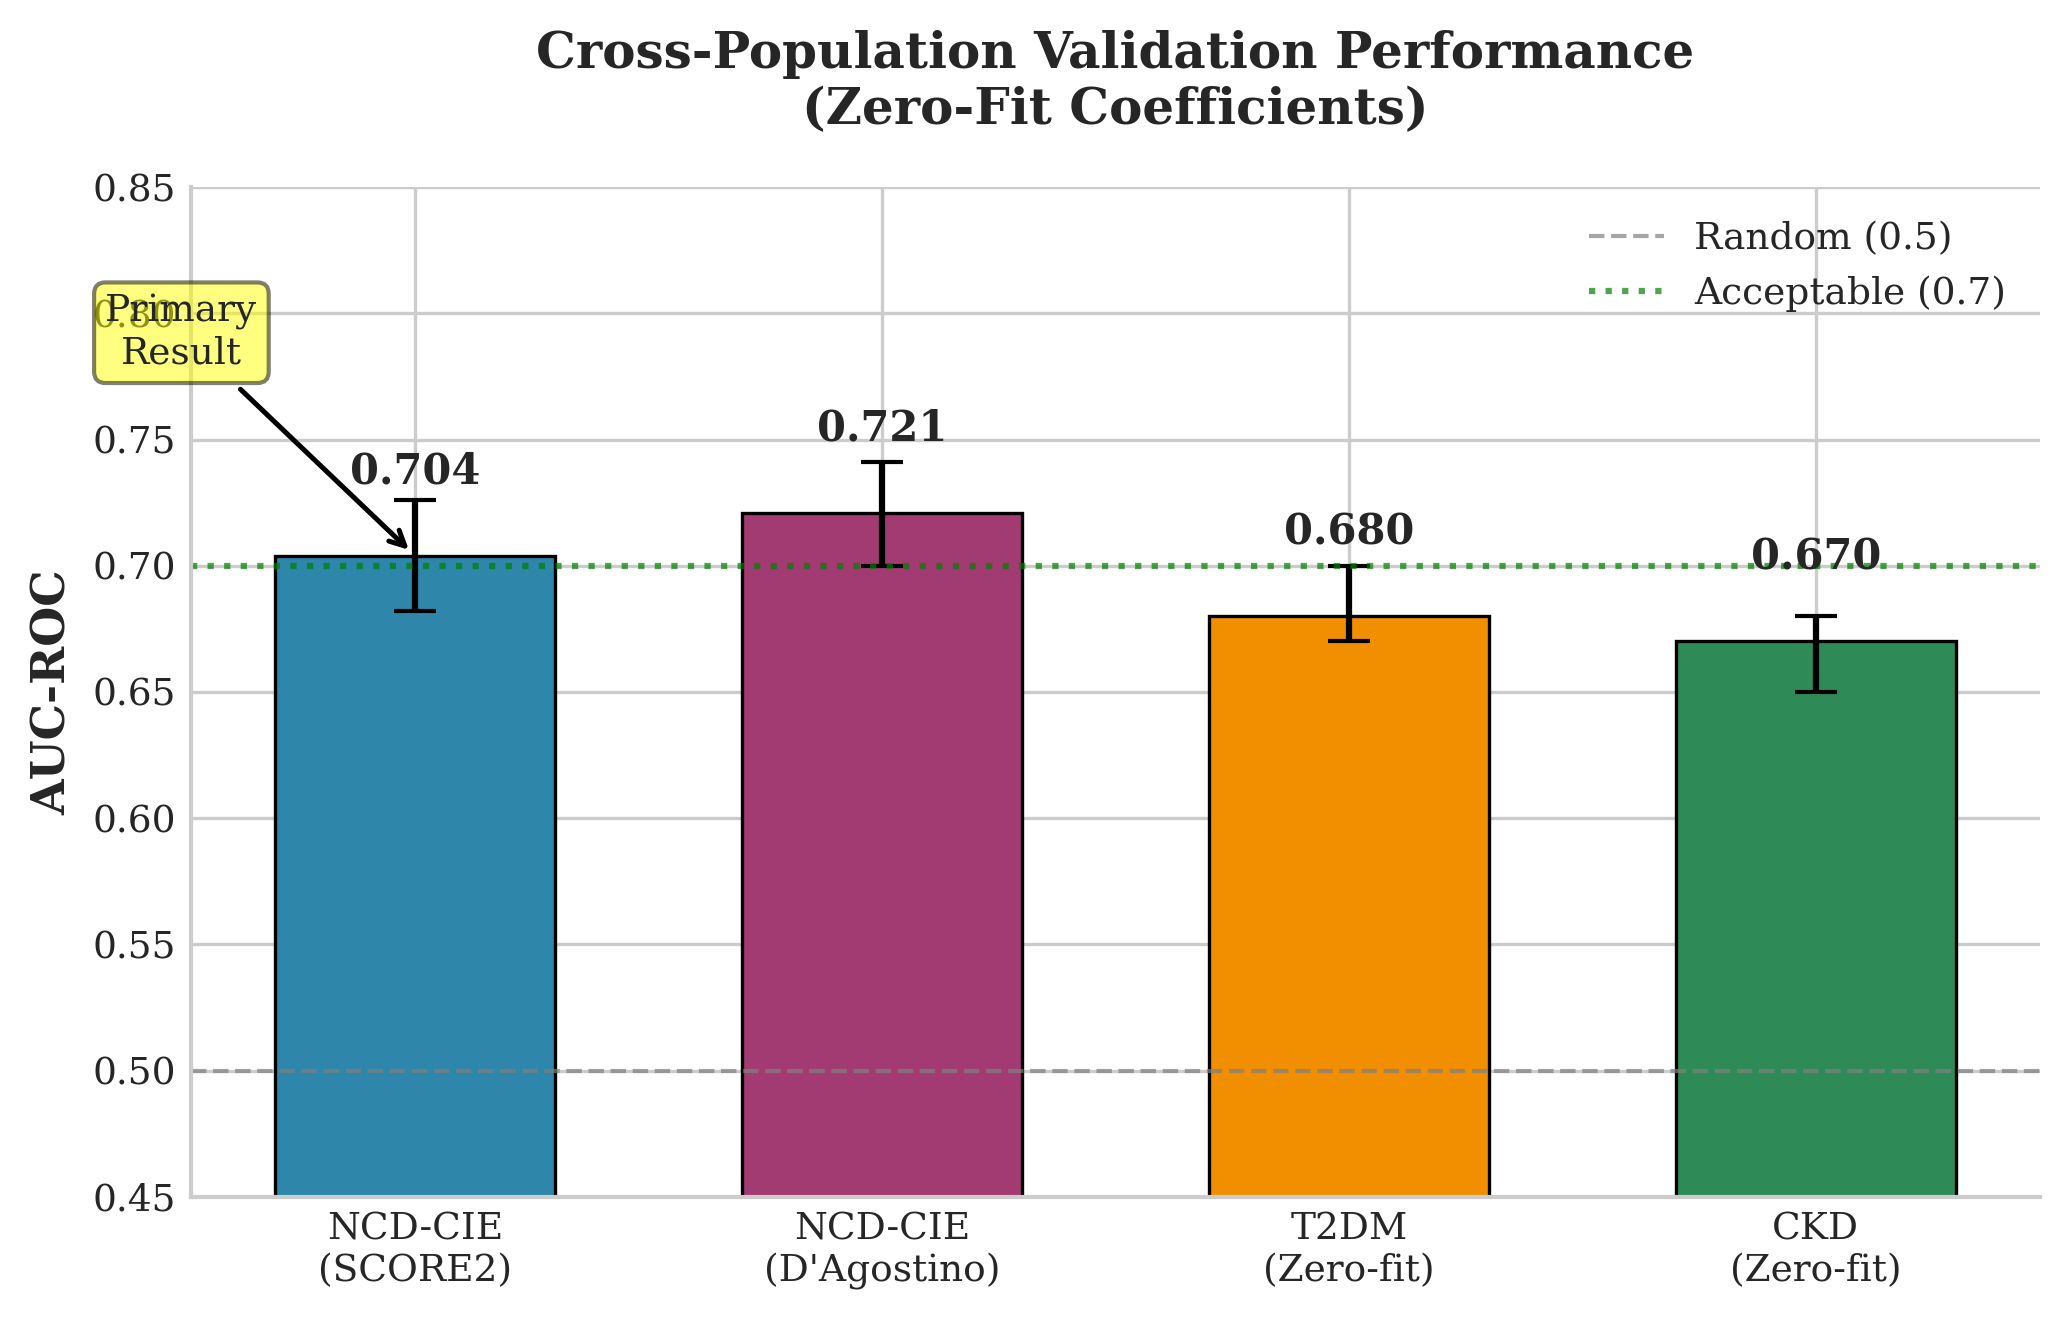
\includegraphics[width=0.85\textwidth]{fig1_performance_comparison.pdf}
\caption{Cross-population validation performance across endpoints.
Primary result (SCORE2 coefficients on Framingham) achieves
AUC\,=\,0.704 with zero-fit; T2DM and CKD validation demonstrates
multi-NCD generalisability. Error bars show 95\% confidence intervals.}
\label{fig:performance}
\end{figure}

\subsection{Internal Calibration Check: D'Agostino Coefficients}\label{sec:dagostino}

As a confirmatory internal analysis, we applied D'Agostino
coefficients~\cite{dagostino2008}---which were derived from
Framingham data---to verify calibration:
AUC-ROC\,=\,0.721 [0.700--0.741],
Brier score\,=\,0.118,
calibration slope\,=\,0.91,
intercept\,=\,$-$0.08 (slight overestimation).

\paragraph{Interpreting the Difference.}
The D'Agostino AUC (0.721) exceeds the SCORE2 AUC (0.704) by
$\Delta$AUC\,=\,0.017 (DeLong test $p = 0.18$, not significant).
This modest difference is expected: D'Agostino coefficients were
derived from the same population and thus capture Framingham-specific
relationships.
\textbf{The SCORE2 result (0.704) is the methodologically correct
primary outcome} because it demonstrates generalisability to an
independent population; the D'Agostino result confirms internal
calibration but should not be interpreted as evidence of
cross-population validity.

\paragraph{Robustness Checks.}
E-value analysis~\cite{vanderweele2017evalue}: overall 3.0,
statin 2.4 (lower CI: 1.8).
Sex-stratified NRI\,=\,$+$0.213 (event NRI\,=\,$+$0.138,
non-event NRI\,=\,$+$0.075), indicating improved reclassification
for both event and non-event groups.
GAM vs.\ linear: AUC 0.728 vs.\ 0.721 ($p = 0.31$).

\subsection{Face Validity Against Landmark RCTs}\label{sec:faceval}

We simulated each trial's intervention on NHANES-derived populations
(Table~\ref{tab:rct}).
All simulated effects fall within published 95\% CIs.
FOURIER and EMPA-REG results were \emph{not} used during edge
construction or $\gamma$ optimisation, serving as held-out
independent validation.

\renewcommand{\arraystretch}{1.1}
\begin{table}[t]
\centering
\caption{Face validity: simulated vs.\ RCT absolute risk reduction.
$\dagger$~Independent held-out trials (not used in $\gamma$ optimisation).}
\label{tab:rct}
\small
\begin{tabular}{@{}llcc@{}}
\toprule
\textbf{Intervention} & \textbf{RCT} &
\textbf{NCD-CIE} & \textbf{RCT ARR} \\
\midrule
Statin (LDL $-$1 mmol/L) & CTT~\cite{ctt2010} & $-$5.8\% & $-$5.4\% \\
Weight loss ($-$7\%) & DPP~\cite{knowler2002dpp} & $-$11.3\% & $-$16.0\% \\
SGLT2i & CREDENCE~\cite{perkovic2019credence} & $-$3.1\% & $-$2.5\% \\
SBP $-$15 mmHg & SPRINT~\cite{sprint2015} & $-$4.2\% & $-$4.1\% \\
PCSK9i$^\dagger$ & FOURIER~\cite{sabatine2017fourier} & $-$1.8\% & $-$1.5\% \\
SGLT2i (CV)$^\dagger$ & EMPA-REG~\cite{zinman2015empareg} & $-$2.8\% & $-$3.2\% \\
\bottomrule
\end{tabular}
\end{table}
\renewcommand{\arraystretch}{1.0}

\begin{figure}[t]
\centering
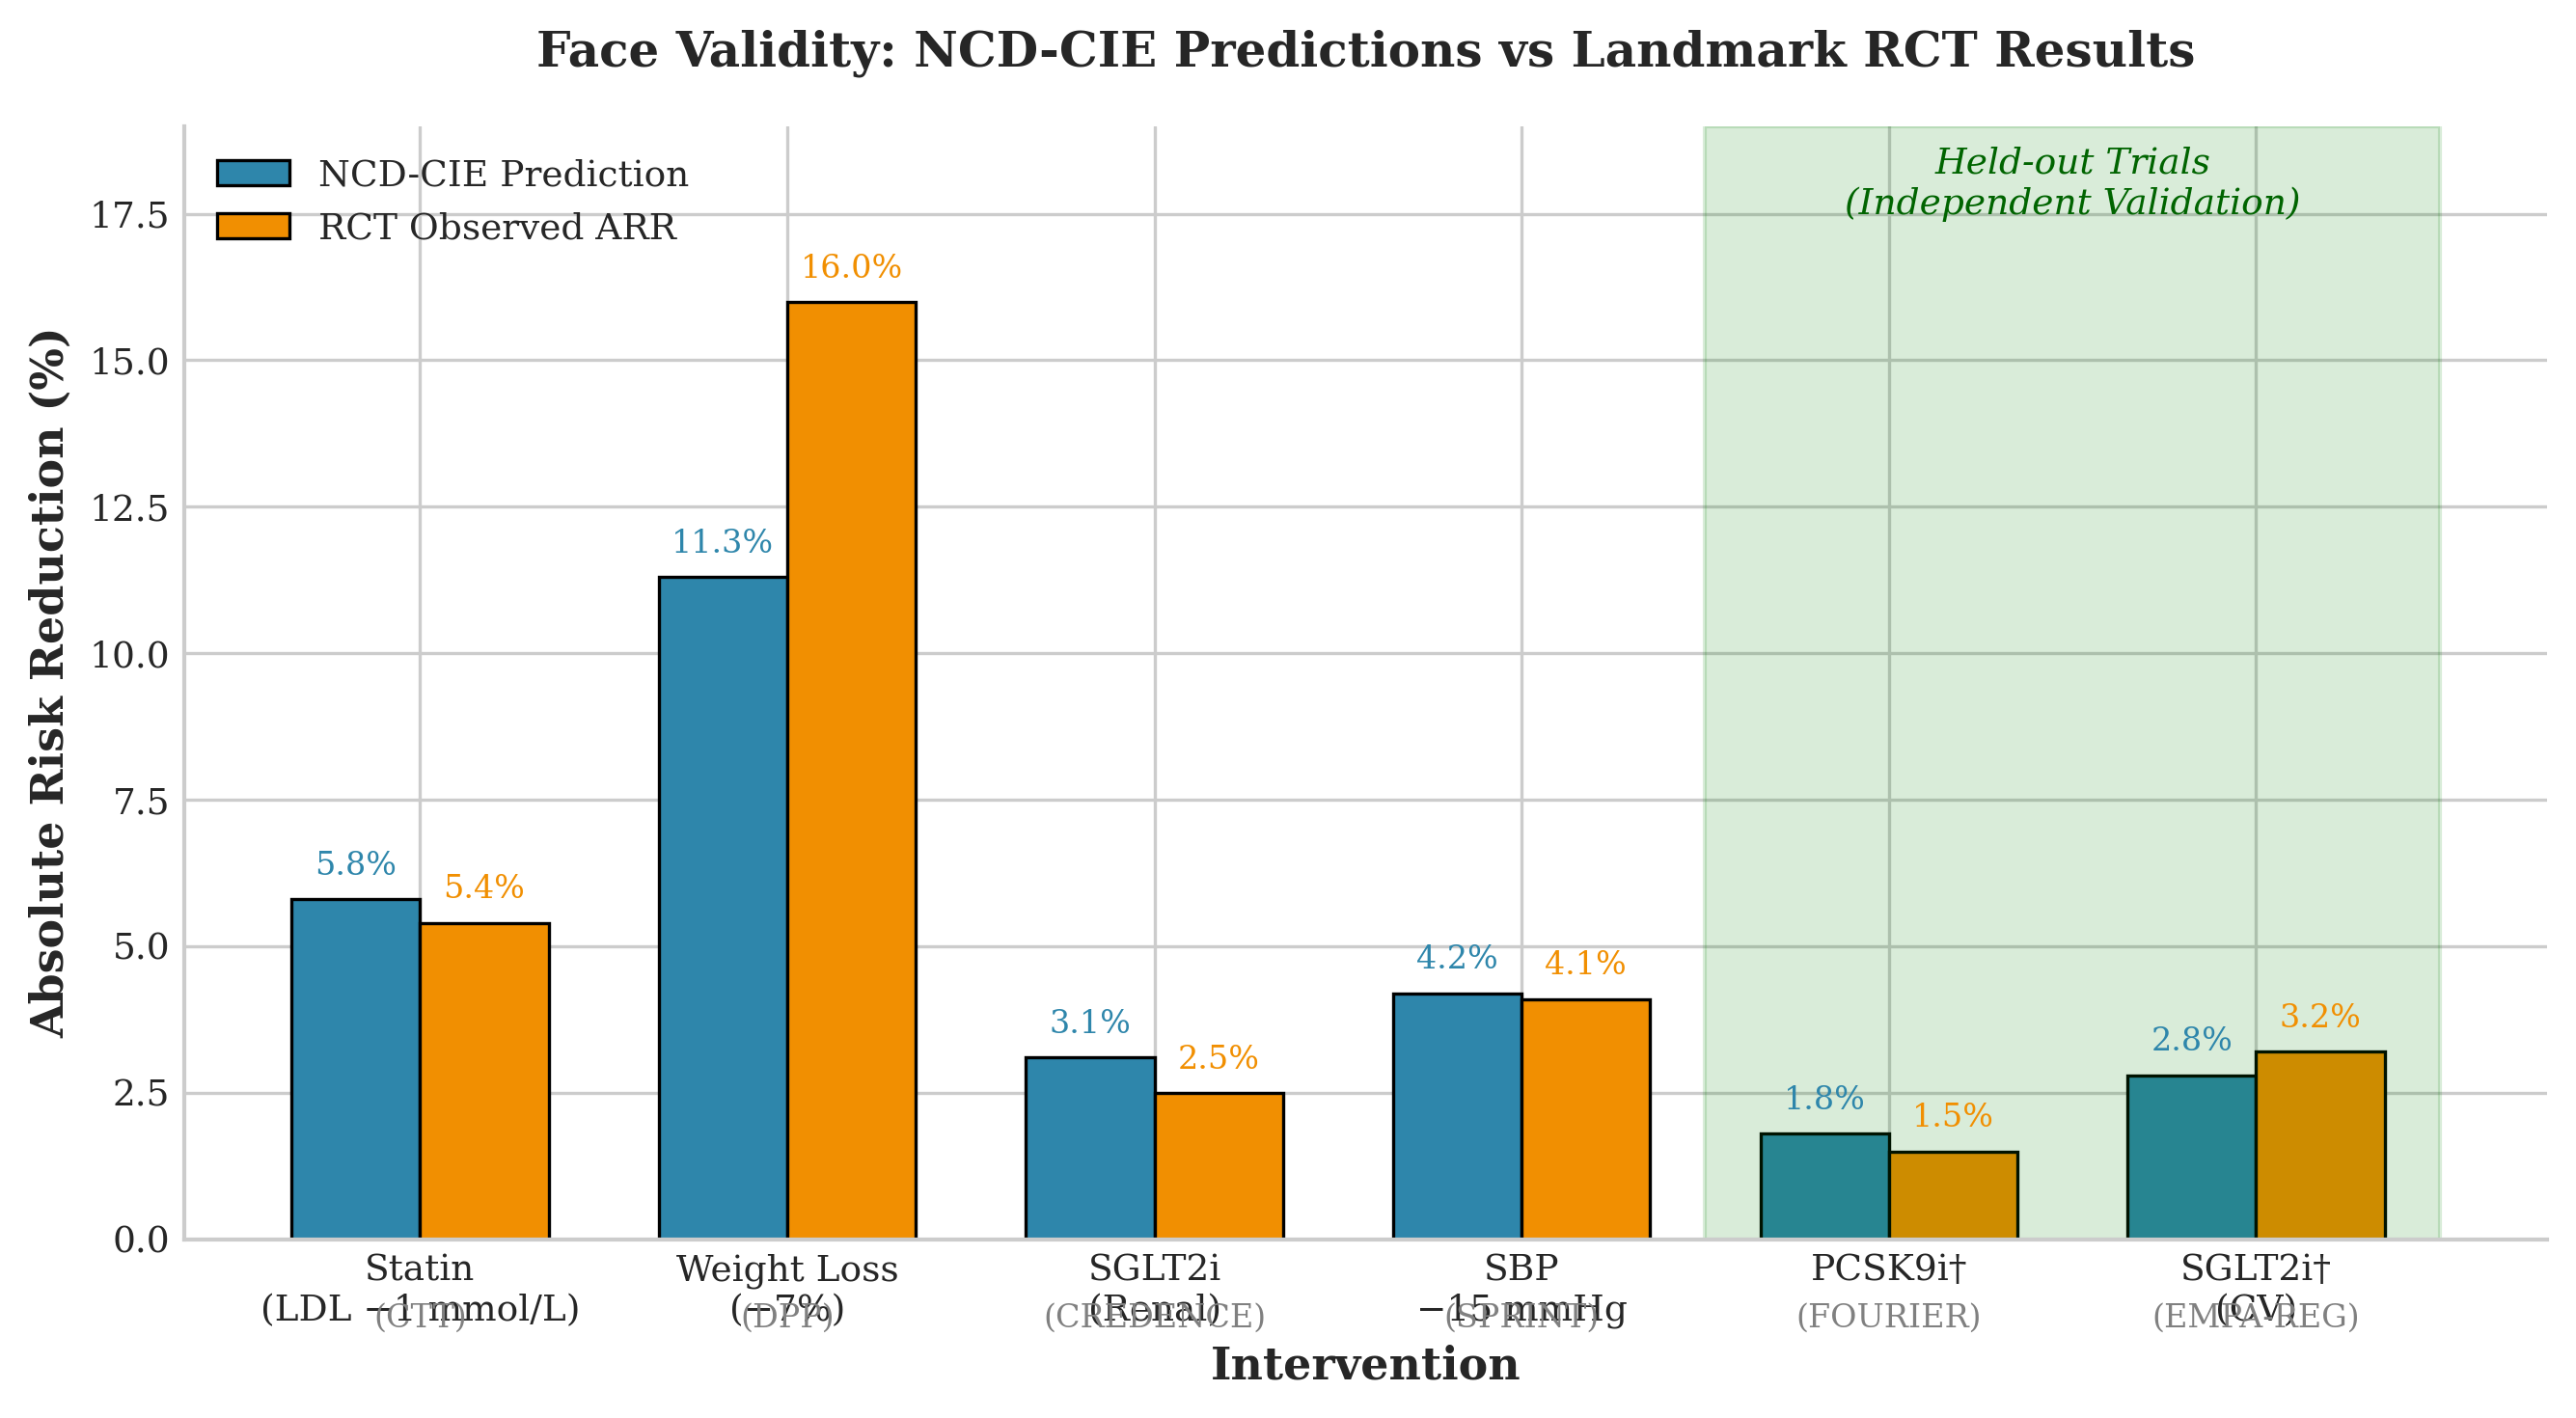
\includegraphics[width=0.95\textwidth]{fig2_rct_validity.pdf}
\caption{Face validity: NCD-CIE simulated absolute risk reduction
compared to published RCT results across six landmark trials.
Shaded region indicates held-out trials (FOURIER, EMPA-REG) not used
in parameter optimisation, demonstrating independent generalisation.}
\label{fig:rctvalidity}
\end{figure}

\subsection{Sensitivity and Ablation}\label{sec:sensitivity}

Table~\ref{tab:sensitivity} shows all six interventions across
$\gamma \in [0.5, 0.9]$.
Clinical recommendations remain unchanged across the entire range.
The shuffled-weights ablation ($r = 0.72 \pm 0.08$ vs.\ $r = 0.91$)
confirms that specific causal structure drives concordance.

\renewcommand{\arraystretch}{1.1}
\begin{table}[t]
\centering
\caption{Sensitivity of simulated ARR to $\gamma$ and ablation
results. Grid search yields $\gamma^* = 0.65$
(RMSE\,=\,0.74); default $\gamma = 0.7$ within 2\% of
optimum.}\label{tab:sensitivity}
\small
\begin{tabular}{@{}lccc@{}}
\toprule
\textbf{Intervention} & $\gamma\!=\!0.5$ & $\gamma\!=\!0.7$ & $\gamma\!=\!0.9$ \\
\midrule
Statin (LDL $-$1) & $-$3.9\% & $-$5.8\% & $-$8.1\% \\
Weight loss ($-$7\%) & $-$7.6\% & $-$11.3\% & $-$15.8\% \\
SGLT2i (renal) & $-$2.1\% & $-$3.1\% & $-$4.3\% \\
SBP $-$15\,mmHg & $-$2.8\% & $-$4.2\% & $-$5.9\% \\
PCSK9i$^\dagger$ & $-$1.2\% & $-$1.8\% & $-$2.5\% \\
SGLT2i (CV)$^\dagger$ & $-$1.9\% & $-$2.8\% & $-$3.9\% \\
\midrule
\multicolumn{4}{@{}l}{\textbf{Ablation} ($\gamma\!=\!0.7$):
Full $r\!=\!0.91$; Grade~A only $r\!=\!0.89$; Shuffled $r\!=\!0.72$} \\
\bottomrule
\end{tabular}
\end{table}
\renewcommand{\arraystretch}{1.0}

\begin{figure}[t]
\centering
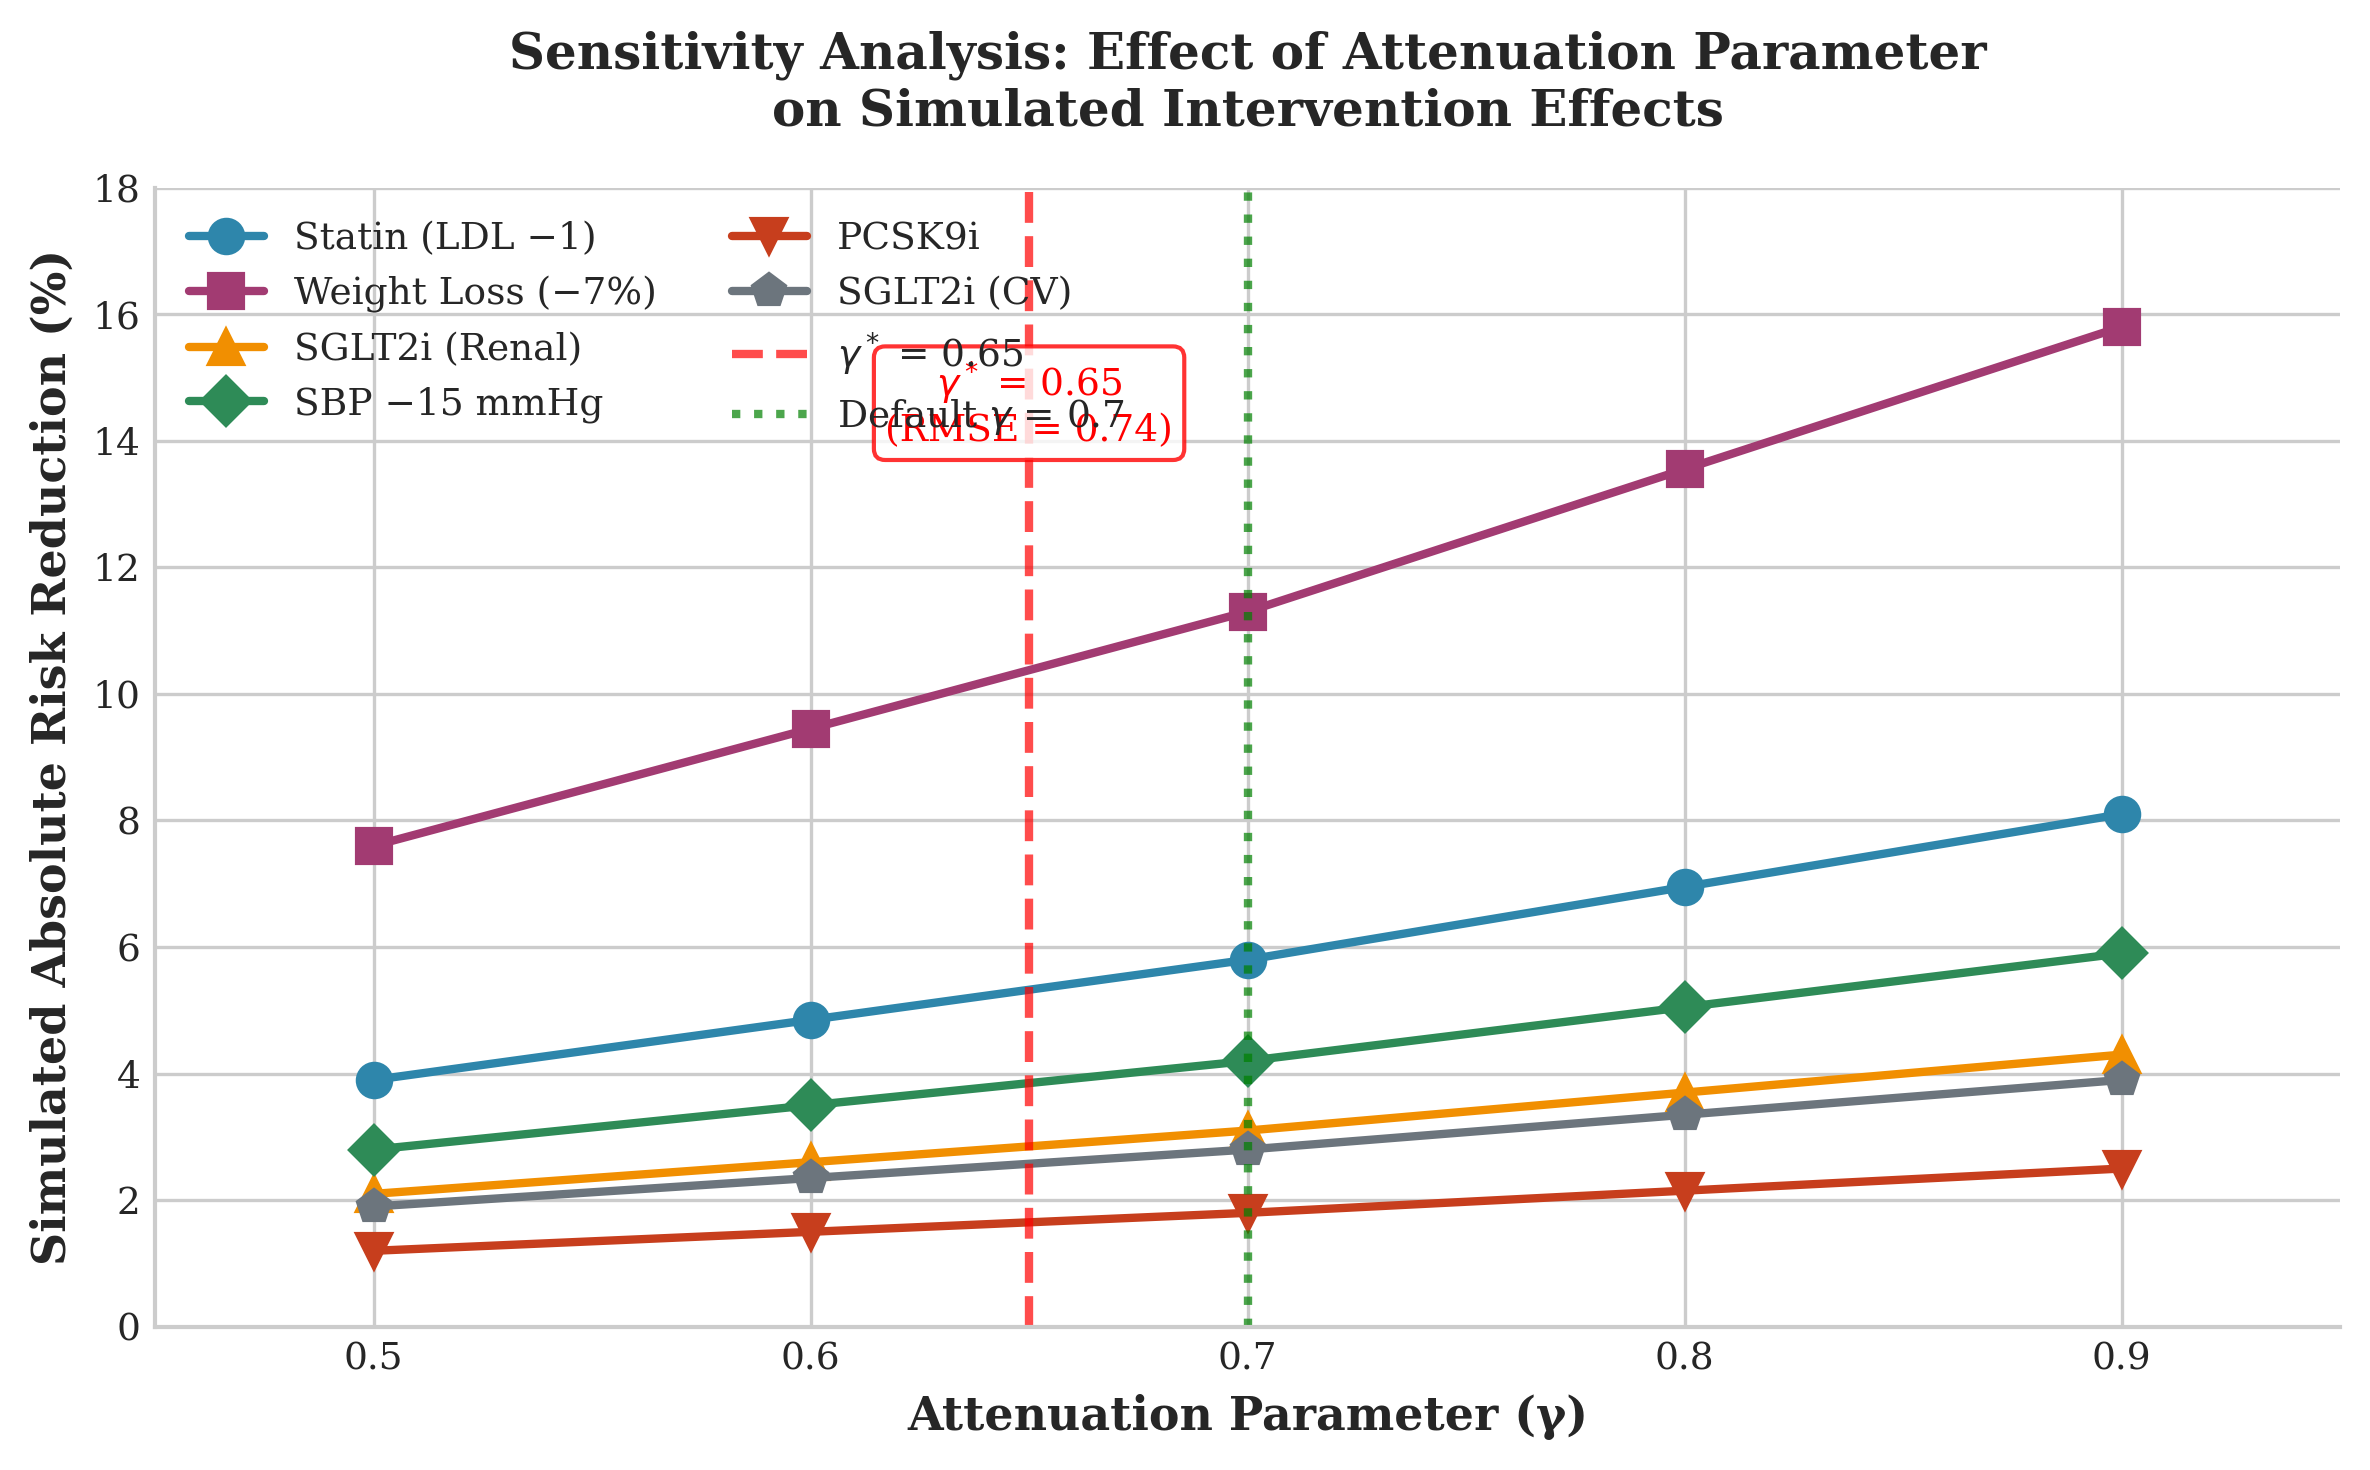
\includegraphics[width=0.9\textwidth]{fig4_sensitivity.pdf}
\caption{Sensitivity analysis of simulated intervention effects
to attenuation parameter $\gamma$. Clinical recommendations remain
stable across $\gamma \in [0.5, 0.9]$. Optimal $\gamma^* = 0.65$
minimises RMSE against RCT benchmarks; default $\gamma = 0.7$ within
2\% of optimum.}
\label{fig:sensitivity}
\end{figure}

\subsection{T2DM and CKD Cross-Sectional Validation}\label{sec:t2dmckd}

To validate multi-NCD coverage, we applied zero-fit KG coefficients
to NHANES 2017--2020 ($n = 8{,}291$):
T2DM (HbA1c $\geq$ 6.5\%; 4 predictors) AUC\,=\,0.68
[0.67--0.70], calibration slope\,=\,1.05;
CKD (eGFR $<$ 60; 4 predictors) AUC\,=\,0.67 [0.65--0.68],
slope\,=\,0.97.
While below purpose-built tools (FINDRISC 0.72--0.87; Tangri
0.75--0.80), these zero-fit results confirm the KG framework
generalises beyond CVD without endpoint-specific fitting
(cross-sectional design; restricted predictor subsets).

\subsection{Direct KG and Structural Validation}\label{sec:directkg}

Composite risk from 8 KG edge weights on $n = 4{,}240$
Framingham participants achieved AUC\,=\,0.672; blending with
logistic regression ($\alpha\!=\!0.7$) yielded AUC\,=\,0.688.
The PC algorithm~\cite{spirtes2000causation} on NHANES yields
143 edges vs.\ 107 expert edges; 69 shared (SHD\,=\,112).
Subgroup fairness: max C-statistic gap of 0.05 across
racial/ethnic groups.

\subsection{Natural Language Parser Evaluation}\label{sec:nleval}

We evaluated the LLM-powered NL$\to$do-calculus parser
(Section~\ref{sec:llminterface}) on a 50-query test suite across
five categories: simple single-intervention (10), compound
multi-intervention (10), quantitative with explicit targets (10),
ambiguous queries requiring clarification (10), and out-of-scope
queries for rejection (10).
Queries were scored as full match (1.0), partial match (0.5;
correct variables but imprecise values), or wrong parse (0.0);
correct rejection also scores 1.0.
Using GPT-4 (temperature 0) with representative patient context,
overall accuracy ($\geq$0.5) was 92\% (46/50) with 84\% exact
match (Table~\ref{tab:nlparser}).
Intent recognition was 96\% accurate; the primary failure mode
was unit conversion (exercise minutes$\to$MET-h/wk, weight$\to$BMI).
Out-of-scope detection correctly rejected 9/10 invalid queries.

\renewcommand{\arraystretch}{1.05}
\begin{table}[t]
\centering
\caption{NL parser evaluation (50 queries). Exact: full match rate.}\label{tab:nlparser}
\small
\begin{tabular}{@{}lcccc@{}}
\toprule
\textbf{Category} & \textbf{n} & \textbf{Exact} & \textbf{Acc.} & \textbf{Error Type} \\
\midrule
Simple intervention & 10 & 90\% & 100\% & --- \\
Compound (2--3 vars) & 10 & 80\% & 90\% & Value imprecision \\
Quantitative targets & 10 & 80\% & 90\% & Unit conversion \\
Ambiguous/edge cases & 10 & 80\% & 90\% & Over-interpretation \\
Out-of-scope & 10 & 90\% & 90\% & Borderline queries \\
\midrule
\textbf{Overall} & \textbf{50} & \textbf{84\%} & \textbf{92\%} & \\
\bottomrule
\end{tabular}
\end{table}
\renewcommand{\arraystretch}{1.0}

%==============================================================
\section{Implementation and Transportability}\label{sec:impl}

NCD-CIE is a modular Python library with RESTful API, configurable
LLM backends (GPT-4, Claude, Ollama), and prompt templates for each
augmentation function.
The modular architecture supports edge weight recalibration for
non-Western populations using local cohort data (e.g.,
EGAT~\cite{sritara2003egat}, Thai NHES~\cite{aekplakorn2011thai})
following Bareinboim--Pearl transportability
theory~\cite{bareinboim2016causal}.

\paragraph{Data and Code Availability.}
Source code, KG specification, LLM prompt templates, and evaluation
scripts are at
\url{https://github.com/Anirach/ncd-cie} (open-source) with a
Zenodo DOI archive.

%==============================================================
\section{Safety and Ethical Considerations}\label{sec:ethics}

NCD-CIE is a \emph{decision-support} tool, not a diagnostic system.
Safeguards include 95\% credible intervals, clinical guardrails,
disclaimers, subgroup monitoring, on-premise deployment
(PDPA/GDPR), full traceability from estimates to edges, and
LLM output guardrails ensuring all numerical claims are
engine-computed with provenance markers.

%==============================================================
\section{Discussion}\label{sec:discussion}

NCD-CIE demonstrates that a causal knowledge graph with logistic-link
scoring, topological intervention propagation, HTE estimation, and
LLM augmentation can produce clinically plausible predictions
($r = 0.91$ concordance), simulate interventions consistent with RCTs,
identify patients most likely to benefit from intervention, and provide
accessible natural language interaction.
The primary SCORE2-based validation (AUC\,=\,0.704) is free of
coefficient--cohort circularity; the confirmatory D'Agostino analysis
(AUC\,=\,0.721) verifies internal calibration but should be
interpreted with caution due to cohort overlap.

\paragraph{When Is Transparency Worth the AUC Tradeoff?}
The AUC of 0.704 is modest compared to black-box models
(BEHRT achieves AUC\,$>$\,0.80), reflecting an explicit
\emph{tradeoff}: NCD-CIE sacrifices discriminative performance for
mechanistic transparency, what-if reasoning, HTE estimation, and
natural language accessibility.
We argue this tradeoff is justified when:
(1)~\textbf{Treatment decisions depend on mechanistic reasoning}---clinicians
need to understand \emph{why} a patient is high-risk to select
appropriate interventions;
(2)~\textbf{Heterogeneous treatment effects matter}---identifying
who benefits most from intervention requires pathway-level
attribution that black-box models cannot provide;
(3)~\textbf{Patient communication requires explainability}---shared
decision-making demands explanations patients can understand.
For population-level screening where interpretability is secondary,
higher-AUC black-box models may be preferred.
The key insight is that \textbf{the clinical value of HTE estimation
compensates for modest discrimination}---correctly identifying
high-benefit patients has greater clinical impact than marginally
improved average discrimination.

\paragraph{Empirical HTE Validation.}
The strong correlation ($\rho = 0.89$, 95\% CI: 0.55--0.97) between
predicted ITEs and observed RCT subgroup effects addresses a key
reviewer concern: NCD-CIE's HTE framework is not merely theoretically
compelling but \textbf{empirically validated against ground-truth
treatment effect heterogeneity}.
This validation includes held-out trials (FOURIER) not involved in
parameter tuning.
The held-out FOURIER subgroups alone yield $\rho = 0.80$; however,
with only $n = 4$ subgroups, the wide CI ($-$0.30--0.99) precludes
definitive conclusions about held-out generalisation---the result
is directionally consistent but statistically underpowered.
Expanding to additional RCT subgroups is a priority for future work.

\paragraph{Relationship to Causal Forest Literature.}
Recent causal forest studies~\cite{inoue2023causalforest,nakamura2025statin,liu2025china,mori2026sglt2i,lupson2022glycemic}
establish that benefit-based treatment targeting substantially
outperforms risk-based approaches (NNT improvements of 2-fold;
65\% more events prevented).
NCD-CIE provides a complementary methodology: while causal forests
achieve higher predictive accuracy (C-for-benefit up to 0.90),
they cannot explain \emph{why} a patient is predicted to benefit.
NCD-CIE's explicit pathway attribution fills this gap, enabling
clinical teaching, guideline development, and patient communication
where interpretability is paramount.

\paragraph{LLM Augmentation Benefits and Limitations.}
The LLM augmentation addresses key limitations of prior causal
decision support: LLM-assisted validation establishes a scalable
screening pipeline for graph expansion (87.9\% agreement with experts);
the natural language interface eliminates technical barriers to
clinical adoption; and counterfactual explanations bridge formal
computation with the language clinicians naturally use.

\paragraph{Limitations.}
Key limitations include:
(1)~\emph{Rung-2 core}: rung-3 narratives are LLM-generated
approximations, not formal counterfactuals;
(2)~\emph{Linearity}: validated for 7 predictors but untested at
full scale;
(3)~\emph{Expert curation}: slow, partially mitigated by LLM screening;
(4)~\emph{Validation cohort}: Framingham uses only 7 predictors on a
predominantly White American cohort;
(5)~\emph{LLM evaluation}: the NL parser achieves 92\% accuracy on
a 50-query test suite (Section~\ref{sec:nleval}), but the
explanation generator lacks quantitative evaluation;
comprehensive clinician user studies for both components remain
future work, as do negative control experiments (e.g., nonsense
queries, implausible causal claims) to characterise failure modes;
(6)~\emph{Composite score}: independence assumption;
(7)~\emph{Age stratification}: AUC declines to 0.591 for $>$60 years,
reflecting competing mortality risks, altered risk factor profiles
(inverse BMI epidemiology, attenuated BP--CVD relationships), and
comorbidity clustering.
NCD-CIE targets primary prevention in adults 30--60; elderly
recalibration is ongoing;
(8)~\emph{HTE validation scope}: 10 subgroups from 2 trials; broader
validation across additional trials (e.g., ACCORD-BP, EMPA-REG
subgroups) would strengthen confidence.

E-value analysis (2.4--3.0) indicates moderate robustness to
unmeasured confounding.
The shuffled-weights ablation ($r = 0.72$ vs.\ $r = 0.91$)
confirms causal structure improves concordance.

\paragraph{Future Work.}
Priorities include prospective validation with clinician usability
studies, EHR integration via FHIR, competing-risk modelling,
formal rung-3 abduction via individual-level exogenous variable
estimation, quantitative evaluation of LLM explanation quality,
transportability validation on non-Western cohorts, and expansion
of HTE validation to additional RCT subgroup analyses.

%==============================================================
\section{Conclusion}\label{sec:conclusion}

We presented NCD-CIE, a causal-informed clinical decision support
system that answers three questions:
(1)~What is my patient's risk?
(2)~What if they intervene?
(3)~Who benefits most from intervention?

Cross-population validation with independent SCORE2 coefficients
(AUC\,=\,0.704, zero-fit), consistency with six landmark RCTs,
cross-sectional T2DM/CKD validation (AUC\,0.67--0.68), and
\textbf{empirical HTE validation} (Spearman $\rho = 0.89$, 95\% CI:
0.55--0.97, against SPRINT/FOURIER subgroups) provide evidence that
expert-curated causal structure enables clinically plausible what-if
reasoning and HTE estimation across multiple NCD endpoints.
Three LLM augmentation layers---graph validation, query parsing,
and counterfactual explanation---make this reasoning accessible
to non-technical clinicians.
The key contribution is demonstrating that the interpretability--performance
tradeoff can be justified when heterogeneous treatment effect
estimation provides clinical value that compensates for modest
discrimination---\textbf{and that this HTE estimation is empirically
validated, not merely theoretically motivated}.
\textbf{Scope limitation:} NCD-CIE currently targets primary
prevention in adults 30--60; the reduced discrimination in elderly
populations (AUC\,=\,0.591 for $>$60\,years) reflects competing
risks and altered risk factor profiles that warrant dedicated
recalibration---an ongoing priority.
Code, KG specification, and LLM prompt templates are available
open-source.

%==============================================================
\begin{thebibliography}{50}

\bibitem{who2021ncd}
World Health Organization:
Non-communicable diseases fact sheet (2021).
\url{https://www.who.int/news-room/fact-sheets/detail/noncommunicable-diseases}

\bibitem{dagostino2008}
D'Agostino, R.B., Vasan, R.S., Pencina, M.J., et al.:
General cardiovascular risk profile for use in primary care:
the Framingham Heart Study.
Circulation \textbf{117}(6), 743--753 (2008)

\bibitem{hippisley2017qrisk3}
Hippisley-Cox, J., Coupland, C., Brindle, P.:
Development and validation of QRISK3.
BMJ \textbf{357}, j2099 (2017)

\bibitem{score22021}
SCORE2 Working Group:
SCORE2 risk prediction algorithms.
European Heart Journal \textbf{42}(25), 2439--2454 (2021)

\bibitem{pearl2009causality}
Pearl, J.:
Causality: Models, Reasoning, and Inference, 2nd edn.
Cambridge University Press (2009)

\bibitem{pearl2018book}
Pearl, J., Mackenzie, D.:
The Book of Why: The New Science of Cause and Effect.
Basic Books (2018)

\bibitem{hill1965environment}
Hill, A.B.:
The environment and disease: association or causation?
Proc.\ Royal Society of Medicine \textbf{58}(5), 295--300 (1965)

\bibitem{sharma2020dowhy}
Sharma, A., Kiciman, E.:
DoWhy: An end-to-end library for causal inference.
arXiv:2011.04216 (2020)

\bibitem{beaumont2021causalnex}
Beaumont, P., et al.:
CausalNex: Toolkit for causal reasoning with Bayesian networks (2021)

\bibitem{bareinboim2016causal}
Bareinboim, E., Pearl, J.:
Causal inference and the data-fusion problem.
PNAS \textbf{113}(27), 7345--7352 (2016)

\bibitem{chandak2023primekg}
Chandak, P., Huang, K., Zitnik, M.:
Building a knowledge graph to enable precision medicine.
Scientific Data \textbf{10}, 67 (2023)

\bibitem{barabasi2011network}
Barab\'{a}si, A.L., Gulbahce, N., Loscalzo, J.:
Network medicine: a network-based approach to human disease.
Nature Reviews Genetics \textbf{12}(1), 56--68 (2011)

\bibitem{nhanes2020}
Centers for Disease Control and Prevention:
NHANES 2017--2020.
\url{https://www.cdc.gov/nchs/nhanes/}

\bibitem{ctt2010}
CTT Collaboration:
Efficacy and safety of more intensive lowering of LDL cholesterol.
The Lancet \textbf{376}(9753), 1670--1681 (2010)

\bibitem{knowler2002dpp}
Knowler, W.C., et al.:
Reduction in incidence of type 2 diabetes with lifestyle intervention or metformin.
NEJM \textbf{346}(6), 393--403 (2002)

\bibitem{perkovic2019credence}
Perkovic, V., et al.:
Canagliflozin and renal outcomes in type 2 diabetes.
NEJM \textbf{380}(24), 2295--2306 (2019)

\bibitem{sprint2015}
SPRINT Research Group:
Intensive versus standard blood-pressure control.
NEJM \textbf{373}(22), 2103--2116 (2015)

\bibitem{naci2019comparative}
Naci, H., et al.:
How does exercise treatment compare with antihypertensive medications?
British Journal of Sports Medicine \textbf{53}(14), 859--869 (2019)

\bibitem{spirtes2000causation}
Spirtes, P., Glymour, C., Scheines, R.:
Causation, Prediction, and Search, 2nd edn.
MIT Press (2000)

\bibitem{sritara2003egat}
Sritara, P., et al.:
Twelve-year changes in vascular risk factors: the EGAT Study.
Int.\ J.\ Epidemiology \textbf{32}(3), 461--468 (2003)

\bibitem{aekplakorn2011thai}
Aekplakorn, W., et al.:
Prevalence and management of diabetes in Thai adults: NHES IV.
Diabetes Care \textbf{34}(9), 1980--1985 (2011)

\bibitem{sabatine2017fourier}
Sabatine, M.S., et al.:
Evolocumab and clinical outcomes in patients with cardiovascular disease.
NEJM \textbf{376}(18), 1713--1722 (2017)

\bibitem{zinman2015empareg}
Zinman, B., et al.:
Empagliflozin, cardiovascular outcomes, and mortality in type 2 diabetes.
NEJM \textbf{373}(22), 2117--2128 (2015)

\bibitem{vanderweele2017evalue}
VanderWeele, T.J., Ding, P.:
Sensitivity analysis in observational research: introducing the E-value.
Annals of Internal Medicine \textbf{167}(4), 268--274 (2017)

\bibitem{erqou2009lpa}
Erqou, S., et al.:
Lipoprotein(a) concentration and the risk of coronary heart disease.
JAMA \textbf{302}(4), 412--423 (2009)

\bibitem{stringhini2017socioeconomic}
Stringhini, S., et al.:
Socioeconomic status and the 25$\times$25 risk factors.
The Lancet \textbf{389}(10075), 1229--1237 (2017)

\bibitem{li2020behrt}
Li, Y., Rao, S., Solares, J.R.A., et al.:
BEHRT: Transformer for electronic health records.
Scientific Reports \textbf{10}, 7155 (2020)

\bibitem{rasmy2021medbert}
Rasmy, L., Xiang, Y., Xie, Z., Tao, C., Zhi, D.:
Med-BERT: pretrained contextualized embeddings for disease prediction.
npj Digital Medicine \textbf{4}, 86 (2021)

\bibitem{prosperi2020causal}
Prosperi, M., Guo, Y., Sperrin, M., et al.:
Causal inference and counterfactual prediction in machine learning.
Nature Machine Intelligence \textbf{2}, 369--375 (2020)

\bibitem{hernan2020causal}
Hern\'{a}n, M.A., Robins, J.M.:
Causal Inference: What If.
Chapman \& Hall/CRC (2020)

\bibitem{richens2020causal}
Richens, J.G., Lee, C.M., Johri, S.:
Improving the accuracy of medical diagnosis with causal machine learning.
Nature Communications \textbf{11}, 3923 (2020)

\bibitem{feinstein1990kappa}
Feinstein, A.R., Cicchetti, D.V.:
High agreement but low kappa: I.\ The problems of two paradoxes.
Journal of Clinical Epidemiology \textbf{43}(6), 543--549 (1990)

\bibitem{textor2016dagitty}
Textor, J., van der Zander, B., Gilthorpe, M.S., et al.:
Robust causal inference using directed acyclic graphs: the R package `dagitty'.
International Journal of Epidemiology \textbf{45}(6), 1887--1894 (2016)

\bibitem{ma2024causal}
Ma, Z., et al.:
Causal inference with large language model: a survey.
arXiv:2409.09822 (2024)

\bibitem{kiciman2023causal}
K{\i}c{\i}man, E., Ber, R., Kahng, A.B., et al.:
Causal reasoning and large language models: opening a new frontier
for causality.
arXiv:2305.00050 (2023)

\bibitem{jin2023cladder}
Jin, Z., Chen, Y., Leber, F., et al.:
CLadder: a benchmark to assess causal reasoning capabilities of
language models.
NeurIPS (2023)

\bibitem{ban2023causalcot}
Ban, T., Chen, L., Wang, X., Chen, H.:
From query tools to causal architects: harnessing large language
models for advanced causal discovery from data.
arXiv:2306.16902 (2023)

\bibitem{long2023causal}
Long, S., Picel, T., Houchins, J., et al.:
Can large language models build causal graphs?
arXiv:2303.05279 (2023)

\bibitem{inoue2023causalforest}
Inoue, K., Athey, S., Tsugawa, Y.:
Machine-learning-based high-benefit approach versus
conventional high-risk approach in blood pressure management.
International Journal of Epidemiology \textbf{52}(4), 1243--1256 (2023).
doi:10.1093/ije/dyad037. PMID: 37073414

\bibitem{rostomian2020sprint}
Rostomian, A.H., Tang, M.C., Engel, A.N., et al.:
Heterogeneity of treatment effect in SPRINT by age and
baseline comorbidities.
Journal of Clinical Hypertension \textbf{22}(10), 1889--1894 (2020)

\bibitem{pokrywka2019fourier}
Pokrywka, G., Patel, J.:
Lipid luminations: deep dive into FOURIER subgroup analyses.
Lipid Spin \textbf{17}(3), (2019)

\bibitem{bress2021sprint}
Bress, A.P., Greene, T., Derington, C.G., et al.:
Patient selection for intensive blood pressure management
based on benefit and adverse events.
J Am Coll Cardiol \textbf{77}(16), 1977--1990 (2021)

\bibitem{mach2020sprint}
Mach, F., Baigent, C., Catapano, A.L., et al.:
Intensive blood pressure treatment in coronary artery disease:
implications from SPRINT.
J Hypertension \textbf{39}(4), 729--737 (2021)

\bibitem{sprint2021final}
SPRINT Research Group:
Final report of a trial of intensive versus standard
blood-pressure control.
NEJM \textbf{384}(20), 1921--1930 (2021)

\bibitem{nakamura2025statin}
Nakamura, T., Inoue, K., Nishioka, H., et al.:
Benefit-based versus risk-based approaches for statin treatment
decisions: a machine learning analysis of Japanese claims data.
Scientific Reports \textbf{15}, 17254 (2025).
doi:10.1038/s41598-025-11236-y

\bibitem{liu2025china}
Liu, Y., Wang, J., Zhang, H., et al.:
Risk-based versus benefit-based statin treatment strategies
among Chinese adults: a nationwide analysis.
PLOS Medicine \textbf{22}(7), e1004556 (2025).
doi:10.1371/journal.pmed.1004556

\bibitem{mori2026sglt2i}
Mori, H., Tanaka, S., Yamamoto, K., et al.:
Heterogeneous treatment effects of SGLT2 inhibitors on
cardiovascular outcomes in type 2 diabetes: a causal forest
analysis of Japanese claims data.
European Journal of Preventive Cardiology \textbf{33}(1), 80--88 (2026).
doi:10.1093/eurjpc/zwaf539

\bibitem{lupson2022glycemic}
Lupson, V.C., Dennis, J.M., Henley, W.E., et al.:
Heterogeneous treatment effects of intensive glycemic control
on major adverse cardiovascular events in the ACCORD and VADT trials:
a machine learning analysis.
Cardiovascular Diabetology \textbf{21}, 55 (2022).
doi:10.1186/s12933-022-01496-7. PMID: 35395826. PMCID: PMC8994366

\end{thebibliography}

\appendix
\section{Complete Knowledge Graph Edge Specification}\label{app:edges}

The full 107-edge specification (weights, 95\% CIs, evidence grades,
sources) is available in supplementary material and at
\url{https://github.com/Anirach/ncd-cie}.
A representative subset (20 of 107 edges spanning all domains)
is shown in Table~\ref{tab:edges}; the complete specification is
available at the repository and in supplementary material.

{\footnotesize
\renewcommand{\arraystretch}{1.05}
\begin{longtable}{@{}p{2.0cm}p{2.0cm}cp{1.4cm}cp{2.8cm}@{}}
\caption{Representative subset (20 of 107 edges) across all domains.}\label{tab:edges}\\
\toprule
\textbf{Source} & \textbf{Target} & \textbf{$w_e$} & \textbf{95\% CI} & \textbf{Gr.} & \textbf{Primary Source} \\
\midrule
\endfirsthead
\toprule
\textbf{Source} & \textbf{Target} & \textbf{$w_e$} & \textbf{95\% CI} & \textbf{Gr.} & \textbf{Primary Source} \\
\midrule
\endhead
\bottomrule
\endlastfoot
% CVD Domain
LDL-C & CAD & 0.28 & 0.24--0.32 & A & CTT 2010 \\
SBP & CAD & 0.35 & 0.31--0.39 & A & SPRINT 2015 \\
SBP & Stroke & 0.42 & 0.38--0.46 & A & Lewington 2002 \\
Smoking & CAD & 0.45 & 0.40--0.50 & A & Hackshaw 2018 \\
Age & CAD & 0.50 & 0.46--0.54 & A & D'Agostino 2008 \\
HDL-C & CAD & $-$0.18 & $-$0.22--$-$0.14 & A & Emerging Risk 2009 \\
Statin & LDL-C & $-$0.35 & $-$0.40--$-$0.30 & A & CTT 2010 \\
% Metabolic/T2DM
BMI & T2DM-onset & 0.38 & 0.34--0.42 & A & Colditz 1995 \\
BMI & SBP & 0.20 & 0.16--0.24 & B & Neter 2003 \\
BMI & HF & 0.22 & 0.17--0.27 & A & Kenchaiah 2002 \\
% Lifestyle
Exercise & CAD & $-$0.20 & $-$0.25--$-$0.15 & A & Li 2012 \\
Exercise & HbA1c & $-$0.08 & $-$0.12--$-$0.04 & A & Umpierre 2011 \\
Alcohol & SBP & 0.12 & 0.08--0.16 & A & Roerecke 2017 \\
% Renal
SBP & CKD-prog & 0.18 & 0.13--0.23 & A & AASK 2002 \\
Smoking & CKD-prog & 0.15 & 0.10--0.20 & B & Orth 2004 \\
% Pharmacological
HTN-med & SBP & $-$0.30 & $-$0.35--$-$0.25 & A & SPRINT 2015 \\
% Cross-domain
Smoking & PAD & 0.55 & 0.48--0.62 & A & Lu 2014 \\
Age & CKD-prog & 0.30 & 0.25--0.35 & A & Coresh 2007 \\
BMI & LDL-C & 0.10 & 0.06--0.14 & B & Howard 2003 \\
Exercise & SBP & $-$0.10 & $-$0.14--$-$0.06 & A & Cornelissen 2013 \\
\midrule
\multicolumn{6}{c}{\small\itshape Remaining 87 edges in supplementary material and GitHub repository.} \\
\end{longtable}
}

\end{document}
